\documentclass[11pt,a4paper,twoside]{article}

\usepackage{minted}
\usepackage{times}
\usepackage{amsmath,amsfonts,amssymb,amsthm}
\usepackage{yfonts}
\usepackage{mathtools}
\usepackage{graphicx}
\usepackage{ bbold }
\usepackage[all]{xy}
\usepackage{tikz}

\usepackage{color}


\theoremstyle{plain}
\newtheorem{thm}{Theorem}[subsection] 

\theoremstyle{definition}
\newtheorem{defn}[thm]{Definition}

\theoremstyle{definition}
\newtheorem{lemma}[thm]{Lemma}
\newtheorem{prop}[thm]{Proposition}

\theoremstyle{definition}
\newtheorem{corollary}[thm]{Corollary}

\theoremstyle{definition}
\newtheorem{example}[thm]{Example} 

\theoremstyle{definition}
\newtheorem*{remark}{Remark}

\usepackage[a4paper]{geometry}
\usepackage{amsfonts}
\usepackage{amsthm}
\usepackage{amsmath}
\usepackage{parskip}
\usepackage{mathrsfs}
\usepackage{graphicx}
\usepackage{amssymb}
\usepackage{xtab}

% You need to set the next two items. 
% If you title is long, you may need to adjust the spacing in titlepage.tex
\newcommand{\TheAuthor}{Josef Dean}
\newcommand{\TheTitle}{Foundational Theory for Alternating Homology}

% uncomment exacly one of these
%\newcommand{\TheModule}{\bf M4K8 Scholarly Report}
\newcommand{\TheModule}{\bf MA4K9 Dissertation}


% Leave the following three as is
\newcommand{\TheUni}{The University of Warwick}
\newcommand{\TheDept}{Mathematics Institute}
\newcommand{\TheSubDate}{\monthyear \formatdate{5}{4}{2016}}

% The are a lot of things you might find useful and want to uncomment. 
% Most things you will want to uncomment or change will be near the top.

% standard maths symbols (you probably want to uncomment all of these)
% \newcommand{\Z}{\ensuremath{\mathbb{Z}}}% integers
% \newcommand{\N}{\ensuremath{\mathbb{N}}}% natural numbers
% \newcommand{\R}{\ensuremath{\mathbb{R}}}% real numbers
% \newcommand{\C}{\ensuremath{\mathbb{C}}}% complex numbers

% Others 
%\newcommand{\st}{\ensuremath{:}}% such that
%\newcommand{\Tau}{\ensuremath{\mathcal{T}}}
%\newcommand{\Nat}{\mathbb{N}}

%\usepackage[numbers]{natbib}% round braces, sort multiple citations
%\usepackage{hyperref}% creates hypertext links in pdf files (natbib compatible)
\usepackage{setspace}
\usepackage{fancyhdr}
%\usepackage{mathrsfs}
%\usepackage{textcomp}
%\usepackage{color}
%\usepackage{graphicx}
%\usepackage{framed}
% \usepackage{algorithmic}% format pseudocode
%\usepackage[vlined,boxed,commentsnumbered,algochapter]{algorithm2e}
% \usepackage[chapter]{algorithm}% float wrapper for algorithms
%\usepackage{amsmath}% American Mathematical Society macros - essential!
%\usepackage{amssymb}% contains amsfonts
%\usepackage{amsthm}% allows more flexibility with theorems
\usepackage[nodayofweek]{datetime} % change the format of printed dates (no american style!) 
%\usepackage{ifdraft}% perform operations conditional on the draft option

% \usepackage{mathptmx}
% \usepackage{mathpazo}
%\usepackage{amscd}
% \usepackage{xy}
% \usepackage{diagxy}
%\usepackage{diagrams}

%\usepackage{marginnote}
%\usepackage{rotating}
%\usepackage{multirow}
% \usepackage{polski}
% \usepackage[T1]{fontenc}
% \usepackage{tikzpicture}
% \usetikzlibrary{matrix,arrows}

% \usepackage[inline]{showlabels}
%\usepackage{booktabs}

% Date format

% Use the datetime package
\newdateformat{monthyear}{\monthname[\THEMONTH], \THEYEAR}% new date format

% New commands, operators and symbols

% Operators
%\DeclareMathOperator{\Sym}{Sym}% symmetric group
%\DeclareMathOperator{\Alt}{Alt}% alternating group
%\DeclareMathOperator{\Id}{Id}
%\DeclareMathOperator{\Hom}{Hom}
%\DeclareMathOperator{\Grp}{Grp}
%\DeclareMathOperator{\supp}{supp}
%\DeclareMathOperator{\fix}{fix}
%\DeclareMathOperator{\dep}{dep}
%\DeclareMathOperator{\lcm}{lcm}
%\DeclareMathOperator{\Aut}{Aut}
%\DeclareMathOperator{\Inn}{Inn}
%\DeclareMathOperator{\Out}{Out}
% \DeclareMathOperator{\dim}{dim}
%\DeclareMathOperator{\Syl}{Syl}
%\DeclareMathOperator{\Hall}{Hall}
%\DeclareMathOperator{\pCore}{pCore}
%\DeclareMathOperator{\Char}{char}
%\DeclareMathOperator{\Image}{Im}
%\DeclareMathOperator{\Ker}{Ker}
%\DeclareMathOperator{\Hcf}{hcf}
%\DeclareMathOperator{\GL}{GL}
%\DeclareMathOperator{\Pc}{Pc}
%\DeclareMathOperator{\Stab}{Stab}
%\DeclareMathOperator{\Orbit}{Orbit}


% Hyphenation fixes
%\newcommand{\letdash}[1]{$#1$\nobreakdash-\hspace{0pt}}% for n-element, k-transitive etc
%\newcommand{\numdash}{\nobreakdash--}

% Sequences
%\newcommand{\seqfin}[3]{\ensuremath{#1_{#2}, \dotsc , #1_{#3}}}
%\newcommand{\seqinf}[3]{\ensuremath{#1_{#2}, #1_{#3}, \dotsc}}

% New environments

% Dedication
%\newenvironment{dedication}
%{\clearpage \thispagestyle{empty} \vspace*{\stretch{1}} \begin{center} \em}
%{\end{center} \vspace*{\stretch{3}} \clearpage}


% Page Layout

% Dimensions
% The guidlines for margins given by the Graduate School are as follows:
% left - no less than 4cm
% right - sufficient for trimming (?)
% top - no less than 1.5cm
% bottom - no less than 1.5cm
% See http://www2.warwick.ac.uk/services/academicoffice/gsp/current/presentation/
% Use the geometry package to set this up
\geometry{includehead,includefoot,left=3cm,right=2cm,top=2cm,bottom=1.5cm}% head and foot are included in total body so that nothing is printed out of the boundaries of the set margins

% Header and footer
% Use the fancydr package
%\ifdraft{%
%\fancypagestyle{plain}{% redefine plain pagestyle for draft
%\renewcommand{\headrulewidth}{0pt}% no head rule in draft mode
%\fancyhf{}% clear headers and footers
%\fancyhead[C]{\ifdraft{DRAFT}{}}% print DRAFT across top if the draft option is set
%\fancyfoot[C]{\thepage}% usual page numbering
%

\pagestyle{fancy}
%\renewcommand{\chaptermark}[1]{\markboth{\thechapter.\ #1}{}}% compact with no capitalisation
%\renewcommand{\sectionmark}[1]{\markright{\thesection.\ #1}}% compact with no capitalisation
%\ifdraft{\renewcommand{\headrulewidth}{0pt}}{}% no head rule in draft mode
\setlength{\headheight}{15pt}
%\fancyhf{}% clear all header and footer fields
% one-sided printing, so no E,O distinction need be made
%\fancyhead[C]{\ifdraft{DRAFT}{}}% print DRAFT across top if the draft option is set
%\fancyhead[R]{\thepage}% page in top right
%\fancyhead[L]{\ifdraft{}{\leftmark}}% chapter number and title in top left

% Theorems
%
%\newtheorem{prop}{Proposition}[thm]
%\newtheorem{lemma}[prop]{Lemma}
%\newtheorem{conjecture}[prop]{Conjecture}
%\newtheorem{theorem}[prop]{Theorem}
%\newtheorem{hyp}[prop]{Hypothesis}
%\newtheorem{cor}[prop]{Corollary}
%\newtheorem{claim}[prop]{Claim}
%newtheorem{remark}[prop]{Remark}
%\newtheorem{notation}[prop]{Notation}
%\newtheorem{defn}[prop]{Definition}


% Numbering
%\numberwithin{equation}{chapter}% standard style numbering, nothing special here


% Algorithms

% Use the algorithms package.
% \renewcommand{\algorithmicrequire}{\textbf{Input:}}
% \renewcommand{\algorithmicensure}{\textbf{Output:}}
% \renewcommand{\algorithmiccomment}[1]{/* #1 */}
%\RestyleAlgo{boxruled}
%\SetAlgoInsideSkip{medskip}
%\setlength{\algomargin}{2em}
%\setlength{\interspacetitleboxruled}{0.7em}
%\setlength{\interspacetitleruled}{0.7em}
%\LinesNumbered
%\SetAlCapNameSty{sc}
%\SetFuncSty{sc}

%\newenvironment{spacedalgorithm}{\begin{algorithm}\onehalfspacing}{\end{algorithm}}
% \newenvironment{onehalfverbatim}{\onehalfspacing\begin{verbatim}}{\end{verbatim}}

%\reversemarginpar
%\newcounter{nootje}
%\setcounter{nootje}{1}
%\renewcommand\check[1]{[*\thenootje]\marginnote{\tiny\begin{minipage}{40mm}\begin{flushright}\thenootje
%: #1\end{flushright}\end{minipage}}\addtocounter{nootje}{1}}


% Document details


\raggedbottom

\DeclareMathOperator{\Ima}{Im}
\DeclareMathOperator{\Ker}{Ker}
\DeclareMathOperator{\Tor}{Tor}
\DeclareMathOperator{\Rank}{Rank}
\DeclareMathOperator{\co}{\!\colon\!}
\DeclareMathOperator{\Alt}{Alt}
\DeclareMathOperator{\sgn}{sgn}
\DeclareMathOperator{\supp}{supp}
\DeclareMathOperator{\diam}{diam}
\DeclareMathOperator{\coloneqq}{\vcentcolon=}

%\renewcommand{\qedsymbol}{$\blacksquare$}

\newcommand*\circled[1]{\tikz[baseline=(char.base)]{
            \node[shape=circle,draw,inner sep=1pt] (char) {#1};}}
            
            



\begin{document}

\pagenumbering{roman}
\begin{titlepage}
\begin{center}

\includegraphics[width=5cm]{Warwick_Crest} 
% this graphic file should live in the working directory
% the size of the following arguments to vspace were determined by 
% trial and error, and produce suitable output for the A4 pagesize.

\vspace*{20pt}
\begin{spacing}{2}
\begin{center}
{\Large \bf \TheTitle} % declared in preamble.tex

\vspace*{14pt}

by

{\Large \bf \TheAuthor} % declared in preamble.tex

\vspace*{16pt}

{\large \bf \TheModule} % declared in preamble.tex

Supervised by David Mond

Submitted to \TheUni % declared in preamble.tex

%\vspace*{36pt}
{\Large \bf \TheDept} % declared in preamble.tex

\TheSubDate % declared in preamble.tex

\vspace*{36pt}

\includegraphics[width=5cm]{warwick_logo} 
% this graphic file should live in the working directory

\end{center}
\end{spacing}
\end{center}
\end{titlepage}

\setcounter{page}{2}
%\renewcommand{\contentsname}{Table of contents}
\tableofcontents
\cleardoublepage
\onehalfspacing
\pagenumbering{arabic}
\onehalfspacing




\section{Introduction}
Our motivation for studying the alternating homology of a space comes from \cite{Goryunov} and \cite{HoustonTopology}.
For map $f\!:\!X\longrightarrow Y$ between spaces $X$ and $Y$, Houston defines the $k^{th}$ multiple point space as
$$D^k(f)=closure\{(x_1,\dots,x_k)\in X^k\mid f(x_1)=\dots=f(x_k) \text{ for } x_i\neq x_j \text{ whenever } i\neq j\}.$$
$S_k$ acts on $D^k(f)$ by permuting copies of $X$, i.e. $\sigma(x_1,\dots,x_k)=(x_{\sigma(1)}\dots,x_{\sigma(k)})$ for $\sigma\in S_k$.
There is a natural projection map that drops the last copy of $X$, 
$$\pi_k\!:\!D^k(f)\longrightarrow D^{k\!-\!1}(f), \quad \quad \pi_k((x_1,\dots,x_{k\!-\!1},x_k))=(x_1,\dots,x_{k\!-\!1})$$ 
giving induced map $\pi_{k\#}\!:\!C_\bullet(D^k(f))\longrightarrow C_\bullet(D^{k\!-\!1}(f))$. The loss of a coordinate cannot take an \emph{alternating} chain (defined properly in the following sections) to a non-alternating chain, so we may restrict to the subcomplex of alternating chains $\pi_{k\#}\!:\!C^{alt}_\bullet(D^k(f))\longrightarrow C^{alt}_\bullet(D^{k\!-\!1}(f))$.

%takes alternating chains to alternating chains by the following argument. We may 'lift' any $\sigma\in S_{k\!-\!1}$ to a $\overline{\sigma}\in S_k$ with the same sign by letting it fix the extra element $k$. This gives $\sigma\pi_k(x_1,\dots,x_k)=(x_{\sigma(1)},\dots,x_{\sigma(k\!-\!1)})=\pi_k\overline{\sigma}(x_1,\dots,x_k)$, so for $c_k\in C^{alt}_l(D^k(f))=\{c\in C_l(D^k(f))\mid \tau\# c=\sgn(\tau)c,\,\,\forall\tau\in S_k\}$ and $c_{k\!-\!1}\coloneqq\pi_{k\#}(c_k)$, we have $$\sigma(c_{k\!-\!1})=\sigma\pi_k(c_k)=\pi_k\overline{\sigma}(c_k)=\pi_k\sgn(\overline{\sigma})c_k=\sgn(\overline{\sigma})\pi_k(c_k)=\sgn(\overline{\sigma})c_{k\!-\!1}=\sgn(\sigma)c_{k\!-\!1}$$
With this morphism of chain complexes and the normal boundary map $\partial$ on singular chains one may write out a double complex
\begin{displaymath}
\xymatrix@R=0.6cm{
& \vdots \ar[d] & \vdots \ar[d] & \vdots \ar[d] & \\
\dots \ar[r]^{\partial\quad\quad} & C_{n\!+\!1}^{alt}(D^{k+1}(f)) \ar[r]^\partial \ar[d]^{\pi_{k+1\#}}  & C_{n}^{alt}(D^{k+1}(f)) \ar[r]^{\partial\quad} \ar[d]^{\pi_{k+1\#}}  & C_{n\!-\!1}^{alt}(D^{k+1}(f)) \ar[r]^{\quad\quad\partial} \ar[d]^{\pi_{k+1\#}}  & \dots \\
\dots \ar[r]^{\partial\quad\quad} & C_{n\!+\!1}^{alt}(D^{k}(f)) \ar[r]^\partial \ar[d]^{\pi_{k\#}}  & C_{n}^{alt}(D^{k}(f)) \ar[r]^{\partial\quad} \ar[d]^{\pi_{k\#}}  & C_{n\!-\!1}^{alt}(D^{k}(f)) \ar[r]^{\quad\quad\partial} \ar[d]^{\pi_{k\#}}  & \dots \\
\dots \ar[r]^{\partial\quad\quad} & C_{n\!+\!1}^{alt}(D^{k-1}(f)) \ar[r]^\partial \ar[d]  & C_{n}^{alt}(D^{k-1}(f)) \ar[r]^{\partial\quad} \ar[d] & C_{n\!-\!1}^{alt}(D^{k-1}(f)) \ar[r]^{\quad\quad\partial} \ar[d] & \dots \\
& \vdots & \vdots & \vdots &
}
\end{displaymath}
Goryunov describes how the spectral sequence of this double complex gives a method for computing the homology of the image of map $f$.
%into a sum of the alternating parts of the homology of the sets $D^k(f)$.

This dissertation aims to carefully prove some of the assertions in the preliminaries of \cite{HoustonTopology}, and to develop tools to better understand and compute alternating homology as a standalone object. In section \ref{Sec:FoundationalTheory} we closely mimic Hatcher's approach to ordinary homology from chapter 2 of \cite{algebraictopology} to build the foundational theory for alternating homology from the ground up. In section \ref{Sec:LinksToOtherTheory} we consider some ways alternating homology may be linked to other, better understood theory.





\section{Building Foundational Theory}
\label{Sec:FoundationalTheory}



\subsection{Introduction to Alternating Homology}
\label{Sec:AlternatingSingularHomology}
The definition of alternating homology is straightforward to anybody with experience of ordinary homology.
Throughout this report, for topological space $X$ we let $C_n(X)$ denote the group of singular $n$-chains,
and $C_{\bullet}(X)$ the chain complex obtained from the boundary operator on simplices. Then $H_n(X)$ is 
the $n^{th}$ Homology group of $X$.

\begin{defn}
Take topological space $X$ on which the symmetric group $S_k$ acts. Then we define the \emph{Alternating Singular Chain Group}
$$C_{n}^{alt}(X) \coloneqq \{ c \in C_n(X) \mid \sigma_\#(c) = \sgn(\sigma)c \quad \forall \,\sigma \in S_k\}$$
where $\sigma_\#:C_n(X)\rightarrow C_n(X)$ denotes the map induced by $\sigma$. When the distinction between the action on $X$ and on its chain group is clear, we will sometimes just write $\sigma$ for $\sigma_\#$.
\end{defn}

\begin{lemma}
\label{AlternatingSingularChainComplex}
The Alternating Singular Chain Groups of $X$ form a chain complex under $\partial$, the ordinary boundary map on simplices, and thus we may define the \emph{ Alternating Homology Groups} 
$H_{n}^{alt}(X)$.
\end{lemma}
\begin{proof}
Firstly, $C_n^{alt}(X)$ is clearly an abelian group. For any $n\geq0$, and $c,d\in C_n^{alt}(X)$\\
(Identity)$\quad\sigma_\#(0) = 0 = \sgn(\sigma) 0 \quad \forall \,\sigma \in S_k$ \\
(Inverse)$\quad\sigma_\#(c) = \sgn(\sigma)c  \implies \sigma_\#(-c) = \sgn(\sigma)(-c)$ \\
(Closure)$\quad\sigma_\#(c+d) = \sigma_\#(c) + \sigma_\#(d) = \sgn(\sigma)c + \sgn(\sigma)d = \sgn(\sigma)(c+d)$\\
Associativity and being abelian are inherited from $C_n(X)$.\\
Next we see that for $c \in C_n^{alt}(X)$, since $\sigma_\# \circ \partial = \partial \circ \sigma_\#$, we have 
$$\sigma_\#(\partial c) = \partial \sigma_\#(c) = \partial (\sgn(\sigma)c) = \sgn(\sigma)\partial c$$
hence $\partial(C_n^{alt}(X)) \subset C_{n-1}^{alt}(X)$. It is already known that $\partial \circ \partial = 0$, so we have chain complex
$$\dots \overset{\partial}{\longrightarrow}C_{n+1}^{alt}(X)\overset{\partial}{\longrightarrow}C_{n}^{alt}(X)\overset{\partial}{\longrightarrow}C_{n-1}^{alt}(X)\overset{\partial}{\longrightarrow}\quad \dots \quad \overset{\partial}{\longrightarrow}C_0^{alt}(X)\overset{0}{\longrightarrow}0$$
\end{proof}
\begin{defn}
An \emph{$S_k$-space} is a topological space $X$ together with an action of $S_k$ on $X$.
\end{defn}
The alternating homolgy groups are of course dependant on the action of the symmetric group on the space, so we use the definition of an $S_k$-space to package them up together. In all our computations we aim to state the action explicitly so as to avoid confusion. 


\begin{defn}
For chain groups $C_\bullet(X)$ on which $S_k$ acts, define map

\begin{center}$\Alt\co C_\bullet(X)\longrightarrow C_\bullet^{alt}(X)\quad$ by $\quad \Alt(c)=\underset{\sigma\in S_k}{\sum}\sgn(\sigma)\sigma(c) $ \end{center}
\end{defn} 
Then $\tau(\Alt(c))=\underset{\sigma\in S_k}{\sum}\sgn(\sigma)\tau\sigma(c)=\underset{\tau^{-1}\sigma\in S_k}{\sum}sgn(\tau^{-1}\sigma)\sigma(c)=\sgn(\tau)\Alt(c)\quad \forall\, \tau\in S_k$,
which is why $\Ima(\Alt)\subset C_n^{alt}(X)$. We shall see soon that this map needn't be surjective, but if we treat it with care it is the obvious way of choosing alternating chains containing particular simplices.

\begin{example}
\label{twoPointSpace}
Let $X=\{x_1,x_2\}$ be the $S_k$-space of two points with the discrete topology. The action of $S_2=\{1,\tau\}$ on $X$ is such that $x_1$ \& $x_2$ are permuted by $\tau$ and fixed by $1$. Allowing $x_1$ and $x_2$ to also denote the obvious choice of constant singular $n$-simplices on $X$ for any $n\geq0$, we see that 
\begin{center}$\Alt(x_1)=x_1-x_2\quad$ and $\quad\Alt(x_2)=x_2-x_1$\end{center}
We can check these chains generate $C_n^{alt}(X)$ explicitly.
\begin{alignat*}{3}
&n_1x_1+n_2x_2\in C_n^{alt}(X) &\iff &\tau(n_1x_1+n_2x_2)=sign(\tau)(n_1x_1+n_2x_2)\\
&&\iff & n_1x_2+n_2x_1=-n_1x_1-n_2x_2\\
&&\iff & n_1 = -n_2
\end{alignat*}
This means the $\Alt$ map is surjective here, so each alternating chain group $C_n^{alt}(X)$ is generated by the alternating $n$-chain $(x_1-x_2)$, giving chain complex
$$\dots\overset{0}{\longrightarrow}\langle x_1-x_2\rangle\overset{1}{\longrightarrow}\langle x_1-x_2\rangle\overset{0}{\longrightarrow}\langle x_1-x_2\rangle\overset{1}{\longrightarrow}\langle x_1-x_2\rangle\overset{0}{\longrightarrow}\langle x_1-x_2\rangle\overset{0}{\longrightarrow}0$$ 
The boundary maps marked as '1' take generators in dimension $n$ to generators in dimension $n-1$, thus $$H_n^{alt}(X)=\begin{cases} \mathbb{Z}  & n=0\\0 & n\neq0 \end{cases}$$
\end{example}


\begin{example}
\label{onePointSpace}
Why was the first example we considered the space of two points, rather than the simpler case $X=\{x\}$, a single point? If we fix any action of some $S_k$ on $X$ we see that it must be trivial, so if $k>1$ there will be a transposition $\sigma$ fixing every simplex $c$ on $X$. Then  $\sigma(c)\!=\!c\!\neq\!\sgn(\sigma)c$, so every alternating chain group is $0$ and the alternating homology of a point is trivial.

This serves to illustrate a difference between ordinary homology and alternating homology. For $X=\bigcup_\alpha X_\alpha$ where each $X_\alpha$ is a path connected component of $X$, we know $H_n(X)\cong\oplus_\alpha H_n(X_\alpha)$. However, if we consider example \ref{twoPointSpace},
$$H_0^{alt}(\{x_1,x_2\})\cong\mathbb{Z}\,\ncong\,0= H_0^{alt}(\{x_1\})\oplus H_0^{alt}(\{x_2\})$$
In fact we may already consider these two incomparable, as $S_2$ will have to act on the spaces differently. We will come to see that path components are no longer the atomic building blocks as they were in ordinary homology. Instead, the orbits of the action play a more key role.
\end{example}

\vspace{2mm}
\begin{example}
\label{Ex:AltNotSurjective}
In the simple cases covered so far the $\Alt$ map has been surjective. The following demonstrates that in slightly more interesting contexts this might not hold. Let $X$ be the sphere of radius $\sqrt{3}$ embedded in $\mathbb{R}^3$ with centre at the origin. The action is defined on coordinates in $3$-space, $\sigma(x_1,x_2,x_3)\coloneqq(\,\sgn(\sigma)x_{\sigma(1)},\,\sgn(\sigma)x_{\sigma(2)},\,\sgn(\sigma)x_{\sigma(3)}\,)$ for $\sigma\in S_k$. Denoting a constant singular simplex by the coordinate vector of its image we may choose $0$-chain $c=(1,1,1)-(-1,-1,-1)$, being careful to remember that three of the minus signs are for negative coordinates in $\mathbb{R}^3$ and one is a negative coefficient in the chain group. Then $$\sigma(c)=(\sgn(\sigma),\sgn(\sigma),\sgn(\sigma))-(-\sgn(\sigma),-\sgn(\sigma),-\sgn(\sigma))=\sgn(\sigma)c$$
So $c\in C^{alt}_0(X)$. The simplices in $c$ are an orbit of the action, so the preimage of $c$ under $\Alt$ if it exists must be of form $p=n_1(1,1,1)+n_2(-1,-1,-1)$. But then
\begin{alignat*}{3}
c=\Alt(p)= & n_1\Alt((1,1,1))+n_2\Alt((-1,-1,-1)) \\
    & =3n_1((1,1,1)-(-1,-1,-1))+3n_2((-1,-1,-1)-(1,1,1)) \\
    & =3(n_1-n_2)((1,1,1)-(-1,-1,-1)) \\
    & =3(n_1-n_2)c
\end{alignat*}
This has no pair of integer solutions $(n_1,n_2)$, hence $c$ is not in the image of $\Alt$.
\begin{figure}
    \centering
    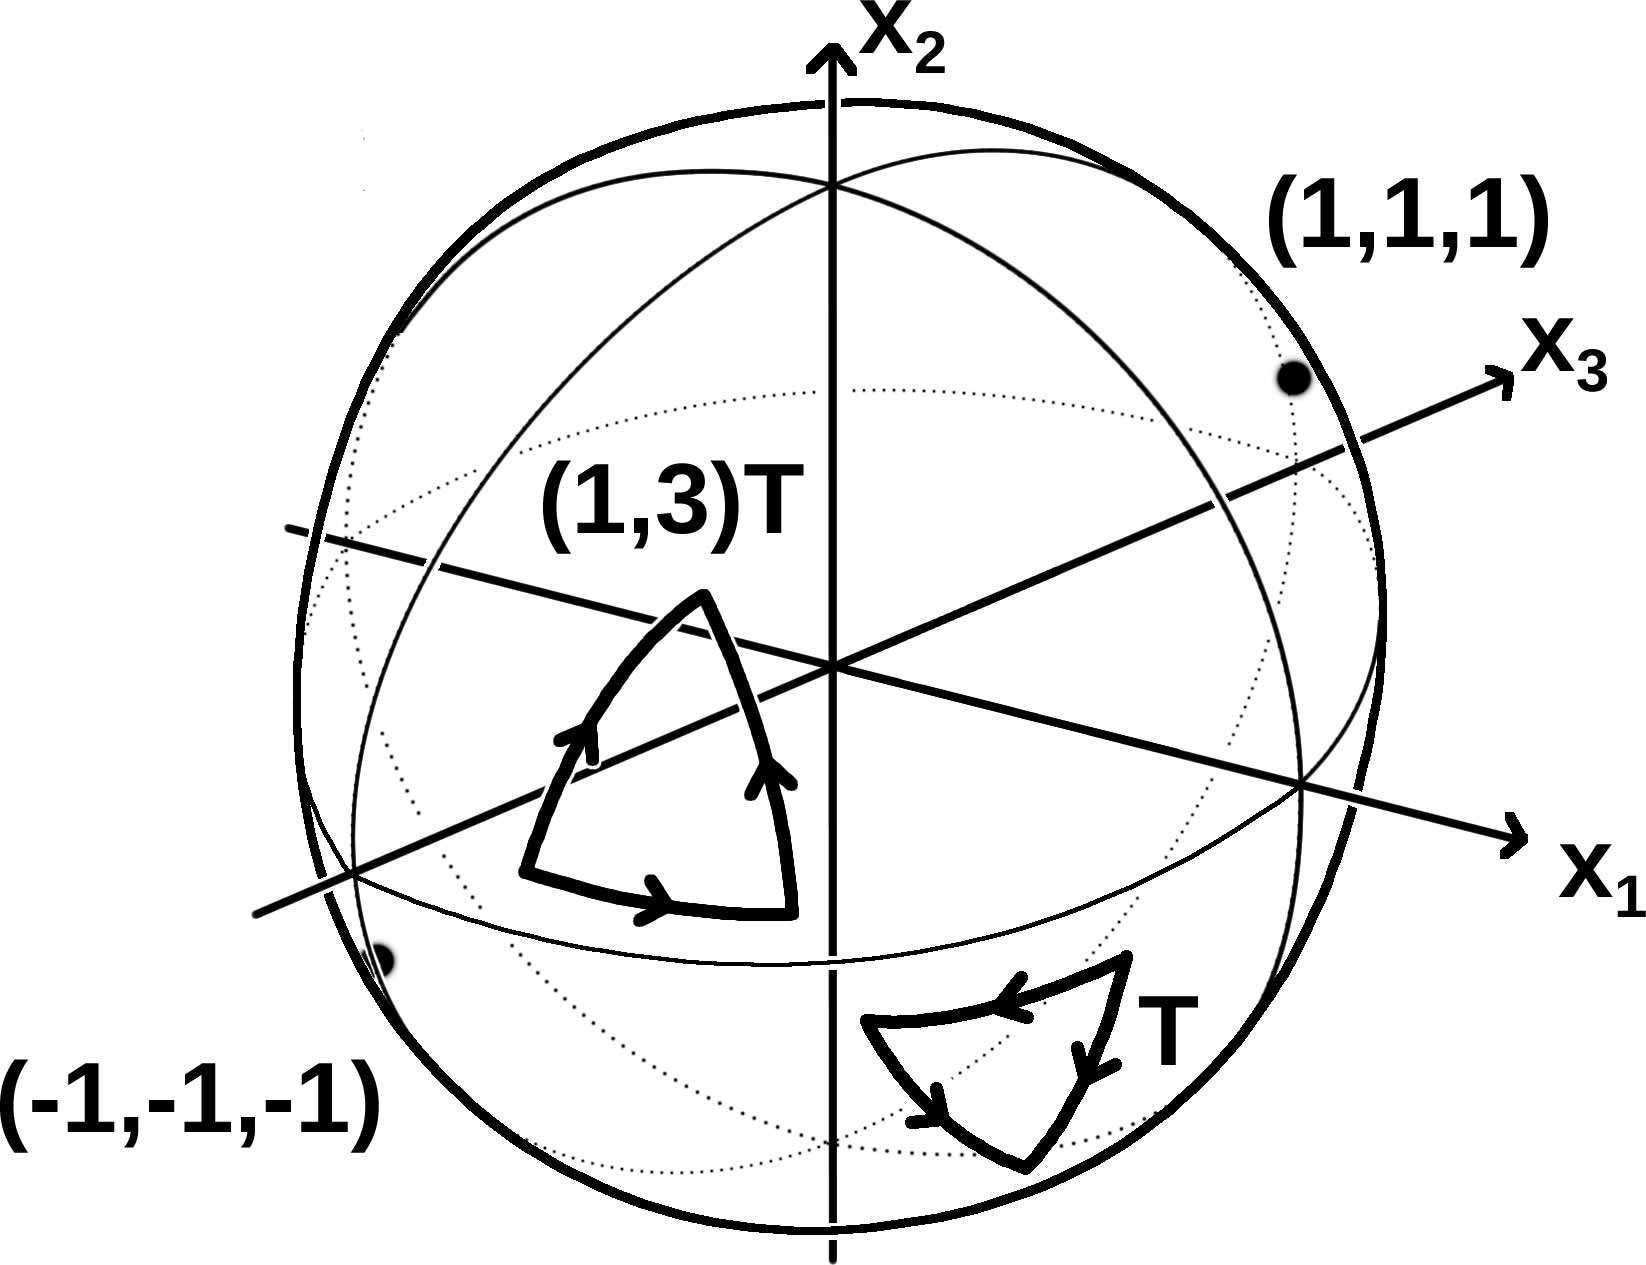
\includegraphics[scale=0.15]{Images/AltNotSurjectiveExample.jpg}
    \caption{The $S_3$-space from example \ref{Ex:AltNotSurjective}, showing the effect of transposition $(1,3)$ on an example triangle $T$, and the points for chain $c$.}
    \label{Fig:AltNotSurjective}
    \end{figure}
\end{example}

\vspace{2mm}

As with ordinary singular homology, this new alternating construction is very difficult to do anything with directly apart from in fairly trivial examples such as \ref{twoPointSpace}. An alternating equivalent to the simplicial homology of a space would be ideal, so that is what we construct next. It will take some time to relate the simplicial construction back to alternating singular homology.




\subsection{Simplicial Alternating Homology}
\label{Sec_AlternatingSimplicialHomology}

\begin{defn}
Given a $\Delta$-complex on $S_k$-space $X$ such that the action on $X$ induces an action on the simplicial chain groups $\triangle_n(X)$, we may define the \emph{Alternating Simplicial Chain Group} to be
$$\triangle_{n}^{alt}(X) \coloneqq \{ c \in \triangle_n(X) \mid \sigma_\#(c) = \sgn(\sigma)c \quad \forall \,\sigma \in S_k\}$$
\end{defn}

\begin{lemma}
The alternating simplicial chain Groups of $X$ form a chain complex under $\partial$, the ordinary boundary map on simplices, and thus we may define the \emph{Simplicial Alternating Homology Groups} 
$H_{n,\triangle}^{alt}(X)$. The proof is exactly the same as \ref{AlternatingSingularChainComplex}.
\end{lemma}

\vspace{2mm}
\begin{example}
\label{Barycentric2Simplex}
To start off simply we might like to look at the simplicial alternating homology of the standard 2-simplex. For $X=\triangle^2$, let $S_3$ act on $X$ as its symmetry group, i.e. transposition $(1,2)$ reflects $X$ across the line of symmetry passing through vertex $v_3$, subsequently permuting vertices $v_1$ and $v_2$. The usual $\Delta$-complex on $X$ is,
$$T=\{[v_1 v_2 v_3],[v_2 v_3],[v_1 v_3],[v_1 v_2],[v_1],[v_2],[v_3]\}$$
\begin{figure}
\centering
\begin{minipage}{.47\textwidth}
  \centering
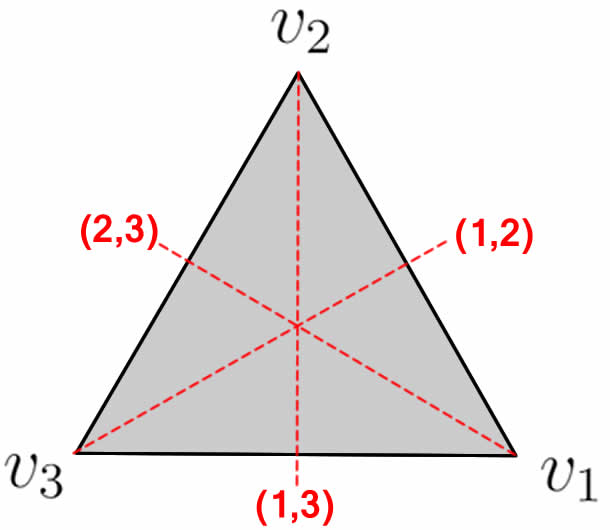
\includegraphics[scale=0.2]{Images/Standard2Simplex.jpg}
\label{S3On2Simplex}
\caption{$S_3$ acting on $\triangle^2$ by permuting corners, or reflecting across lines of symmetry.}

\end{minipage}%
\hfill
\begin{minipage}{.47\textwidth}
  \centering
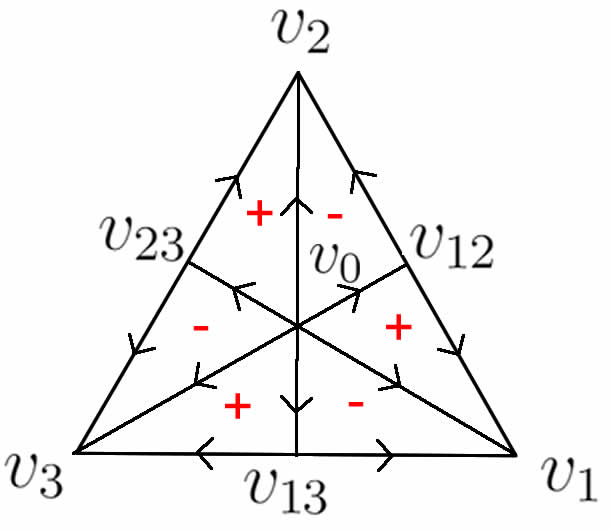
\includegraphics[scale=0.2]{Images/BarySub2Simplex.jpg}
\label{BarySub2Simplex}
\caption{First barycentric subdivision of $\triangle^2$ with signs for an alternating 2-chain.}

\end{minipage}
\end{figure}
where $[v_{i_1},\dots,v_{i_n}]$ denotes the normal map $\triangle^n\longrightarrow X$ taking vertex $m$ to $v_{i_m}$.
If we try to induce an action on the chain groups of this complex, we are faced with problems like $(1,2)[v_1 v_2]=[v_2 v_1]\notin T$, so we're going to need to triangulate $X$ differently. Consider instead the first barycentric subdivision of $\triangle^2$, with $\Delta$-complex
\begin{alignat*}{3}
D =\{ & [v_0 v_{12} v_1],[v_0 v_{12} v_2],[v_0 v_{13} v_1],[v_0 v_{13} v_3],[v_0 v_{23} v_2],[v_0 v_{23} v_3],\\
& [v_0 v_1],[v_0 v_{12}],[v_0 v_2],[v_0 v_{23}],[v_0 v_3],[v_0 v_{13}],[v_{12} v_1],[v_{12} v_2],[v_{23} v_2],[v_{23} v_3],[v_{13} v_1],[v_{13} v_3],\\
&[v_1],[v_2],[v_3],[v_{12}],[v_{23}],[v_{13}]\}
\end{alignat*}

Figure 3 shows the orientations of $D$. Checking by hand, we see that the above action on $X$ induces an action on the chain groups $\triangle_\bullet(X)$, so we may compute the chain groups of simplicial alternating homology.
\begin{alignat*}{3}
\triangle_2^{alt}(X)= & \, \langle [v_0v_{12}v_1]-[v_0v_{12}v_2]+[v_0v_{23}v_2]-[v_0v_{23}v_3]+[v_0v_{13}v_3]-[v_0v_{13}v_1] \rangle\\
\triangle_1^{alt}(X)= & \, \langle  [v_{12}v_1]-[v_{12}v_2]+[v_{23}v_2]-[v_{23}v_3]+[v_{13}v_3]-[v_{13}v_1]\rangle\\
\triangle_0^{alt}(X)= & \, 0
\end{alignat*}The boundary map takes the generator of $\triangle_2^{alt}(X)$ to the generator of $\triangle_1^{alt}(X)$, giving chain complex
\begin{center}
$0\overset{0}{\longrightarrow}\triangle_2^{alt}(X)\cong\mathbb{Z}\overset{1}{\longrightarrow}\triangle_1^{alt}(X)\cong\mathbb{Z}\overset{0}{\longrightarrow}\triangle_0^{alt}(X)\cong0\overset{0}{\longrightarrow}0\quad$ thus $\quad H_{n,\triangle}^{alt}(X)\cong0 \quad\forall\,n$
\end{center}
This is the second example we have seen of a non-empty space having trivial alternating homology (this time simplicial) in dimension $0$, something we don't see in ordinary homology. This will come into play in section \ref{Sec_AlternatingReducedHomology} when we consider the worth of an reduced alternating homology theory.
\end{example}

Example \ref{Barycentric2Simplex} generalises to arbitrary dimension as we will see in example \ref{BarycentricNSimplex}, but before that we need to cover the behaviour of a particular kind of action. In the following lemma we are talking about singular chains, but by the natural map $\triangle_n^{alt}(X)\rightarrow C_n^{alt}(X)$ taking simplices to their characteristic maps, the result holds for simplicial chains.

\vspace{2mm}
\begin{lemma}
\label{PermFix_NonAlt}
For topological space $X$, suppose $S_k$ acts on product space $X^k$ by permuting copies of $X$, where $k\geq 2$. For any $n$-simplex $c$ on $X^k$, if there exists $\sigma\in S_k$ such that $\sigma (c)\!=\!c$ and $\sigma\!\neq\! 1$, then there also exists $\sigma^\prime\in S_k$ an odd permutation such that $\sigma^\prime c=c$. In particular $c$ does not appear in any alternating $n$-chains.
\end{lemma}
\begin{proof}
Take $\sigma \in S_k$ fixing simplex $c\in C_n(X)$. As $\sigma\!\neq\!1$ there exist $i,j\in\{1,...,k\}$ such that $\sigma(i)\!=\!j$ and $i\!\neq\! j$. For all $(x_1,\dots,x_k)\in\Ima(c)\subset X^k$ we have $(x_1,\dots,x_k)=(x_{\sigma(1)},\dots,x_{\sigma(k)})$, in particular $x_i=x_{\sigma(i)}=x_j$, so $\sigma^\prime=(i,j)$ is an odd permutation fixing $c$.

For the last part, take an alternating $n$-chain 
\begin{center}$A=\alpha c + \underset{i}{\sum} \alpha_i c_i,\quad c_i\neq c \quad$ and so $\quad\sigma^\prime(A)=\sgn(\sigma^\prime)A=-A=-\alpha c -\! \underset{i}{\sum} \alpha_i c_i$\end{center}
None of the $c_i$ can map to $c$ under $\sigma^\prime$, as otherwise $c_i\!=\!(\sigma^\prime)^{-1}(c)\!=\!\sigma^\prime(c)\!=\!c\,$. Equating coefficients now gives $\alpha \sigma^\prime(c)\!=\!-\alpha c\implies\alpha c\!=\!-\alpha c\implies\alpha=0$, hence $A$ does not contain $c$.
\end{proof}



\begin{example}
\label{BarycentricNSimplex}
The standard $n$-simplex is a useful building block for more interesting spaces, so we will generalise \ref{Barycentric2Simplex} to any $n\geq0$.

For $X=\triangle^n$ embedded as normal in $\mathbb{R}^{n+1}$, let $S_{n+1}$ act on $X$ by permuting the vertices, i.e. by permuting coordinates of $\mathbb{R}^{n+1}$. We are going to construct a $\Delta$-complex on the first barycentric subdivision of $X$ by specifying an ordering of its vertices.\\
Define the \textbf{level} of a vertex in the subdivision to be one less than the number of non-zero coordinates in its position vector in $\mathbb{R}^{n+1}$. Equivalently and more intuitively, the level of a vertex is the dimension of the simplex in $\triangle^n$ of which it is the barycentre. The level quantifies how central the vertex is.
\begin{figure}
    \centering
    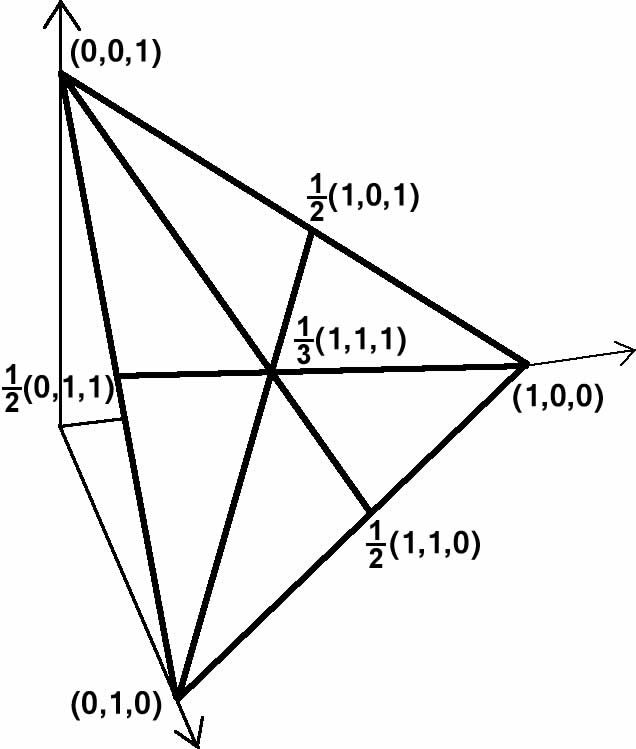
\includegraphics[scale=0.24]{Images/2SimplexInR3.jpg}
    \label{Fig:Triangle2inR3}
    \caption{The first barycentric subdivision of $\triangle^2$ embedded in $\mathbb{R}^3$}
\end{figure}
In figure 4 where $n=2$, the corners have position vectors like $(1,0,0)$ and level $0$. The midpoints of each edge have positions like $\frac12(1,0,1)$ and level $1$. The centre of the face has position $\frac13(1,1,1)$ and level $2$.\\
We represent an $l$-simplex of the subdivision by an ordered list of the position vectors for each vertex, e.g. $[\frac1{3}(1,1,1),(0,0,1)]$ is one of the $1$-simplices in the figure. Then define $D$ to be the set of simplices satisfying the following two criteria.
\begin{enumerate}
    \item The representation lists vertices of the subdivision in strictly decreasing level.
    \item Any coordinate that is zero in a vector must remain zero in subsequent vectors in the list.
\end{enumerate}
See that $D$ uses the level of vertices to put an oriented simplex on each part of the subdivision. The boundary map removes vectors from a list, which preserves condition 1 and 2 and hence maps back into $D$. Similarly, the action of $S_{n+1}$ preserves the level of a vertex by not changing  the total number of zeros in its position vector, and preserves condition 2 by permuting coordinates consistently across all vectors in a list. Thus we have a $\Delta$-complex on $\triangle^n$ on which $S_{n+1}$ acts.

We may now compute the Alternating Simplicial Homology of the space. First consider groups of dimension $0\leq r < n\!-\!1$.\\
Simplex $c\in \triangle_r(X)$ is represented by an ordered list of $r$ vertices in $\mathbb{R}^{n+1}$. There are too few vectors to set each coordinate to $0$ one at a time, so we can find two coordinates that are either never changed throughout the list, or become $0$ in the same vector. A transposition of these two coordinates will fix $c$, and so $c$ is not in $\triangle_r^{alt}(X)$ by lemma \ref{PermFix_NonAlt}. Hence $\triangle_r^{alt}(X)\cong0$.

\begin{minipage}{.3\textwidth}
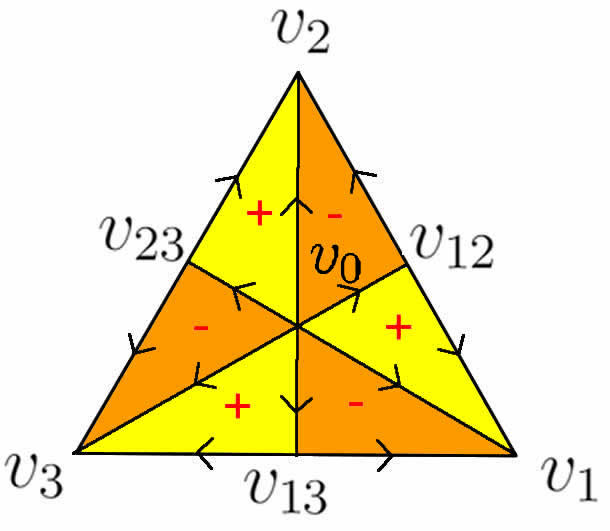
\includegraphics[scale=0.2]{Images/BarySub2SimplexSign.jpg}
\end{minipage}
\begin{minipage}{.70\textwidth}

Next consider simplex $c\in\triangle_n(X)$ which will contain a vertex of every level, starting with $\frac1{n+1}(1,1,\dots,1,1)$ and finishing on one of the outer corners like $(1,0,\dots,0,0)$. There are $(n\!+\!1)!$ different ways of sequentially setting all but one coordinate to $0$ in $\mathbb{R}^{n+1}$, and as such there are $(n\!+\!1)!$ $n$-simplices in $D$. The action of $S_{n+1}$ merely permutes the order in which the choice is made, so all the $n$-simplices are in a single orbit, and hence an alternating chain must contain them all or be trivial.
\end{minipage}
By the freedom of the action on this set, $A\coloneqq\Alt(c)$ is a consistent way of assigning a sign to each of the simplices, so we have $\triangle_n^{alt}(X)=\langle A\rangle\cong\mathbb{Z}$.
 
Finally, in dimension $n-1$, the presentations of simplices are those of the $n$-simplices less one vertex. If the missing vertex is any other than the very first, i.e. $\frac1{n+1}(1,1,\dots,1,1)$, then a jump of two levels is made in the list, so by similar logic to the lower dimensional case, there is a transposition fixing the simplex and it cannot be in an alternating chain. Much as in dimension $n$, the remaining simplices simply correspond to the possible orders in which the coordinates can be set to $0$, the only difference being that the choices start from the very first vector in the list. Once again, we have free action of $S_{n+1}$ on these 'outer face' simplices with a single orbit, so we may make a consistent choice of sign to get a single alternating $(n\!-\!1)$-chain called $B$. This means $\triangle_{n-1}^{alt}(X)\cong\langle B\rangle\cong\mathbb{Z}$ and we have our chain complex.
$$0\longrightarrow \triangle_n^{alt}(X)\cong\mathbb{Z}\overset{\partial}{\longrightarrow}\triangle_{n\!-\!1}^{alt}(X)\cong\mathbb{Z}\longrightarrow0$$
The boundary map $\partial$ takes the generator of $\triangle_n^{alt}(X)$ to the generator of $\triangle_{n\!-\!1}^{alt}(X)$ by the following argument. Summands of the boundary sum that come from deleting the first (level $n$) vertex of an $n$-simplex will be external faces with appropriate sign. Any internal faces produced by the boundary map are fixed by some transposition, so two $n$-simplices differing by that transposition will share the face, canceling each others contributions with their opposing signs. Thus
$$H_{k,\triangle}^{alt}(X)\cong 0$$
\end{example}
\begin{example}
By considering $X$ to instead be the boundary of $\triangle^n$ in the above example, we can use the same construction less anything concerning the centre vertex to find the alternating homology of a space homeomorphic to $S^{n-1}$, acted on by $S_{n+1}$.
$$H_{k,\triangle}^{alt}(\partial\triangle^n)\cong \begin{cases} \mathbb{Z} & k=n-1 \\ 0 & k\neq n-1\end{cases}$$
\end{example}
We don't yet know anything about how alternating homology behaves with respect to homotopy, or even if it is changed by the choice of $\Delta$-complex. Over the next few sections we will closely follow Hatcher's foundational chapter on ordinary homology in \cite{algebraictopology}, and aim to show analogous results arising from our new object.

\subsection{Reduced Alternating Homology}
\label{Sec_AlternatingReducedHomology}
All non-empty spaces have non-trivial homology in dimension 0. Where it is convenient to have the homology groups of a trivial space (a point) be all trivial, the Reduced Homology is introduced through an augmented chain complex\\
\begin{center}$\dots\longrightarrow C_2(X)\overset\partial\longrightarrow C_1(X)\overset\partial\longrightarrow C_0(X)\overset\varepsilon\longrightarrow\mathbb{Z}\longrightarrow 0\quad$ where $\quad \varepsilon(\Sigma_in_n\sigma_i)=\Sigma_in_i$\end{center}
However, as seen in example \ref{onePointSpace}, alternating homology \emph{can} be trivial in dimension $0$ without this change. In fact, suppose we were to construct the same augmented chain complex with alternating chain groups. Take $C_0^{alt}(X)\ni a\!=\! \Sigma_i\alpha_ic_i$, take $\sigma\in S_k$ and define $\sigma(i)=j$ wherever $\sigma(c_i)=c_j$, i.e. define the action of $S_k$ on the indices by $c_{\sigma(i)}=\sigma(c_i)$. If $\sigma$ is a transposition, then
$$\Sigma_i(-\alpha_i)c_i=-\Sigma_i\alpha_ic_i=\sigma(\Sigma_i\alpha_ic_i)=\Sigma_i\alpha_ic_{\sigma(i)}=\Sigma_i\alpha_{\sigma(i)}c_i\quad\implies\quad\alpha_i\!=\!-\alpha_{\sigma(i)}\,\,\forall\,i$$
Thus $\sigma$ being a bijection between the coefficients of $a$ means $\varepsilon(a)=\Sigma_i\alpha_i=0$ for the arbitrary alternating $0$-chain $a$. Clearly this augmented chain complex is not going to tell us anything useful.

Suppose instead we don't blindly put a $\mathbb{Z}$ on the end of the complex, rather we try to mimic the idea behind it. Hatcher offers the perspective that the extra group is in fact the group of empty chains, and that the boundary map takes $0$-chain $[v]$ to empty chain $[\,]$, and in turn maps $[\,]$ to $0$. By definition of the alternating chain group applied to dimension $-\!1$,
$$C_{-\!1}^{alt}(X)\coloneqq\{c\in C_{-\!1}(X)=\langle[\,]\rangle\mid \sigma(c)=\sgn(\sigma)c\quad\forall\,\sigma\in S_k\}$$
How would the action of $S_k$ extend to the group of empty chains? There is one $(-\!1)$-simplex, so the action must be trivial, meaning the alternating relation doesn't hold for any odd permutations and hence $C_{-\!1}^{alt}(X)\cong0$. Thus even from this perspective there is no sensible way to extend the chain complex, so we will not be defining a reduced alternating homology.



\subsection{Homotopy Invariance}
\label{Sec_HomotopyInvariance}
\begin{thm}
Any homotopy equivalence $f\co X\rightarrow Y$ induces isomorphisms $f_*\co H_n(X)\rightarrow H_n(Y)$ on ordinary homology.
\end{thm}
Homotopy invariance is one of the fundamental properties of ordinary homology, and for our new object to have any utility we should hope it behaves similarly. As we shall see however, an additional restriction is required for Hatcher's proof in \cite{algebraictopology} to hold. 

\begin{defn}
If group $G$ ($S_k$ in our case) acts on spaces $X$ and $Y$, then function $f\!:\!X\rightarrow Y$ is called \emph{Equivariant} if 
$$\forall\,g\in G,\,\forall x\in X,\quad f(g\circ x)=g\circ f(x)$$
\end{defn}
\begin{defn}
Two maps $f,g\!:\!X\!\rightarrow\!Y$ are called \emph{$S_k$-Homotopic} if there exists homotopy $F\!:\!X\!\times\! I\!\rightarrow\!Y$ between them such that $F_t\coloneqq F(-,t)\!:\!X\!\rightarrow\!Y$ is equivariant $\forall\,t\in I$. Notice this implies both $f$ and $g$ are also equivariant.
\end{defn}
\begin{defn}
If $X$ and $Y$ are $S_k$-spaces, then map $F\!:X\!\longrightarrow\!Y$ is called an \emph{$S_k$-Homotopy Equivalence} if there exists map $G\!:\!Y\!\longrightarrow\!X$ such that $GF$ is $S_k$-homotopic to $\mathbb{1}_X$ and $FG$ is $S_k$-homotopic to $\mathbb{1}_Y$.
\end{defn}

\begin{thm}\label{EquivariantHomotopyHomomorphism}
If two maps $f,g\!:\!X\rightarrow Y$ are $S_k$-homotopic, then they induce the same homomorphisms $f_*\!=\!g_*\!:\!H_n^{alt}(X)\rightarrow H_n^{alt}(Y)$.
\end{thm}
In particular, if $f\!:\!X\longrightarrow Y$ is an $S_k$-homotopy equivalence with $S_k$-homotopy inverse $h\!:\!Y\longrightarrow X$, then by construction their composition $hf$ is $S_k$-homotopic to $\mathbb{1}_X$ and induces the same isomorphism. Thus, as $(hf)_*=h_*f_*$, we immediately have the following main result of this section.

\vspace{2mm}
\begin{corollary}\label{Cor:SkHomotopyEquivalence}
The $S_k$-homotopy equivalence $f\co X\rightarrow Y$ induces isomorphisms $f_*\co H_n^{alt}(X)\rightarrow H_n^{alt}(Y)$ on alternating homology. \hfill $\blacksquare$
\end{corollary}
We will now give a proof of theorem \ref{EquivariantHomotopyHomomorphism}, largely identical Hatcher's theorem 2.10 but with an equivariant twist. Afterwards we shall explore through some examples why the change is necessary, and what happens if it is not implemented.

\textbf{\emph{Proof of \ref{EquivariantHomotopyHomomorphism}}}.
We start as normal by subdividing $\triangle^n\times I$ into $(n\!+\!1)$-simplices. Let $\triangle^n\times\{0\}=[v_0,\dots,v_n]$ and $\triangle^n\times\{1\}=[w_0,\dots,w_n]$, where $v_i=w_i$ under projection $\triangle^n\times I\rightarrow\triangle^n$. Then our first $(n\!-\!1)$-simplex is $[v_0,\dots,v_n,w_n]$. The next is $[v_0,\dots,v_{n\!-\!1},w_{n\!-\!1},w_n]$, and then we follow this pattern, raising one vertex from $\triangle^n\!\times\!\{0\}$ to $\triangle^n\!\times\!\{1\}$ at a time until we have a collection of $(n\!+\!1)$-simplices covering the whole of $\triangle^n\times I$. Figure 5 depicts cases $n\!=\!1$ and $n\!=\!2$.
\begin{figure}
\centering
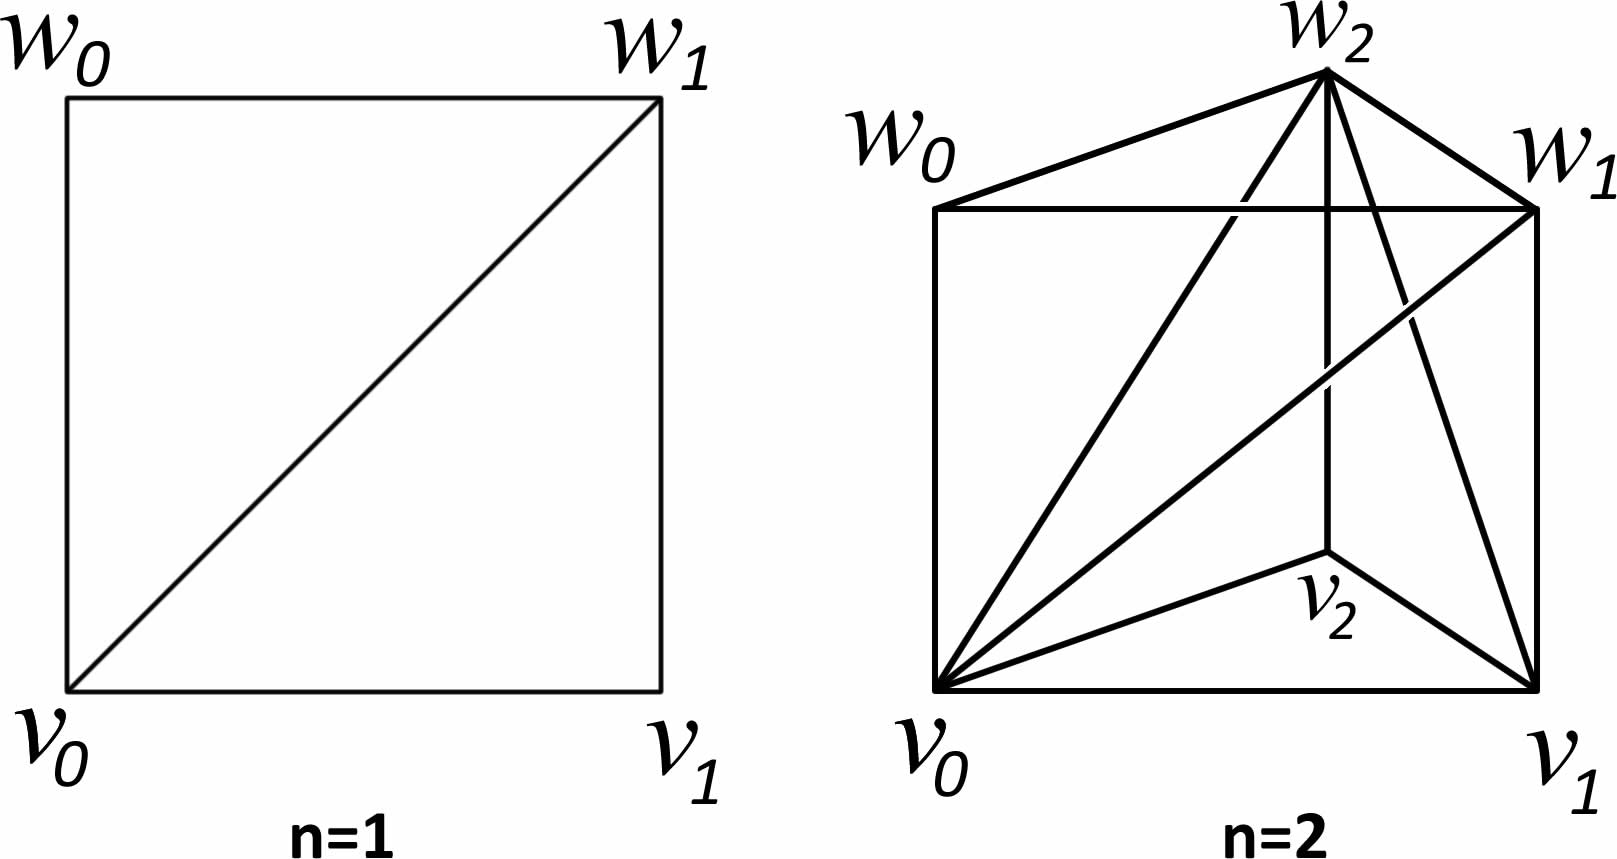
\includegraphics[scale=0.15]{Images/PrismSimplices.jpg}
\label{fig:PrismSimplices}
\caption{Dividing $\triangle^1\times I$ and $\triangle^2\times I$ into simplices}
\end{figure}

Given $S_k$-homotopy $F\!:\!X\!\times\! I\!\rightarrow\!Y$ from $f$ to $g$ and singular simplex $c\!:\!\triangle^n\!\rightarrow\! X$ recall the \emph{Prism Operators}
$$P\!:\!C_n(X)\!\rightarrow\!C_{n\!+\!1}(Y), \quad P(c)=\sum_{i=0}^{n}(-1)^iF\circ(c\times\mathbb{1})|{[v_0,\dots,v_i,w_i,\dots,w_n]}$$
$P$ is extended to the whole of $C_n(X)$ by linearity. We would like to restrict $P$ to $C_n^{alt}(X)$, and require that it then maps into $C_{n\!+\!1}^{\,alt}(Y)$. By choice of $F$, for any $\sigma\in S_k,\,c\in C_n^{alt}(X)$,
\begin{alignat*}{3}
\sigma P(c) &= \sum_{i=0}^{n}(-1)^i\sigma F\circ(c\times\mathbb{1})|[v_0,\dots,v_i,w_i,\dots,w_n] & \\
&      =\sum_{i=0}^{n}(-1)^iF\circ(\sigma(c)\times\mathbb{1})|[v_0,\dots,v_i,w_i,\dots,w_n]  \quad & \text{ ($F$ equivariant)}\\
&      =P(\sigma(c))=P(\sgn(\sigma)c) & \text{($c$ alternating)}\\
&      =\sgn(\sigma)P(c)  & \text{(linearity)}
\end{alignat*}
Hence we can restrict $P\!:\!C_n^{alt}(X)\rightarrow C_{n\!+\!1}^{alt}(Y)$. By the same computations done in the ordinary case, $P$ is a chain homotopy between chain maps $f_\#$ and $g_\#$, namely it satisfies the relation $\partial P =g_\# - f_\#-P\partial$. Looking at figure 5, geometrically this means the boundary of the prism is a signed sum of its top face $\triangle^n\times\{1\}$, bottom face $\triangle^n\times\{0\}$ and the sides $\partial\triangle^n\times I$.

We may now consider any cycle $\alpha\in C_n^{alt}(X)$. As $\partial\alpha =0$, we have
$$g_\#(\alpha)-f_\#(\alpha)=\partial P(\alpha)+P(\partial\alpha) = \partial P(\alpha)$$
Then $g_\#(\alpha)-f_\#(\alpha)$ is the boundary of an alternating chain in $Y$, so $g_\#(\alpha)$ and$f_\#(\alpha)$ determine the same alternating homology class in $H_n^{alt}(Y)$.\hfill$\blacksquare$\\





\begin{example}
\label{NonequivariantHomotopyVariance}
Let us relax just one condition from the above theorem. Suppose we required that the two homotopic maps be equivariant, but that they needn't be homotopic via an equivariant homotopy. Now consider $X=Y=S^1\subset\mathbb{C}$, acted on by $S_2$. Let $\tau$, the non-trivial element of $S_2$, act by reflecting across the same line through the origin in both spaces. Take maps $f,g\!:\!X\rightarrow Y$, where $f$ is the identity and $g$ is a rotation by $\pi$ (see figure 6).

Define  $F\!:\!X\!\times\! I\rightarrow Y$ the (not equivariant) homotopy from $f$ to $g$ by $F(x,t)=xe^{t\pi i}$. Let $x_1,x_2\in X$ be distinct points that reflect onto each other, so $c=x_1-x_2$ is an alternating $0$-chain. If we construct the prism operator using $F$, figure 7 depicts $P(c)$, and it is clearly not an alternating chain, so would be useless in our proof of \ref{EquivariantHomotopyHomomorphism}.
\begin{figure}
\begin{minipage}{.49\textwidth}
\centering
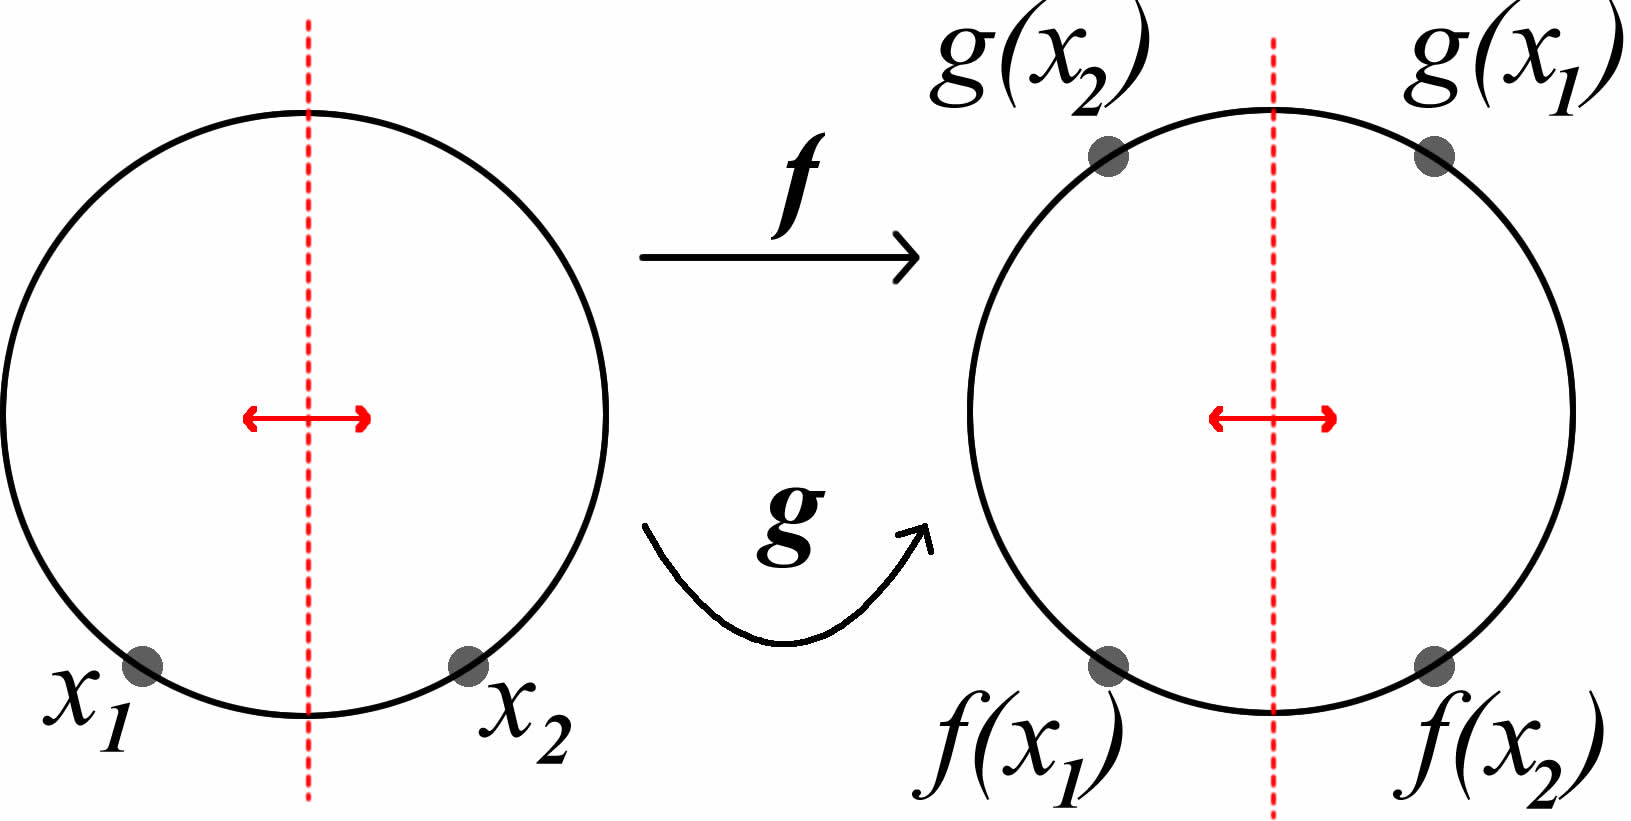
\includegraphics[scale=0.12]{Images/NonEquivariantHomotopy.jpg}
\label{fig:NonEquivariantHomotopy}
\caption{Equivariant maps}
\end{minipage}
\begin{minipage}{.49\textwidth}
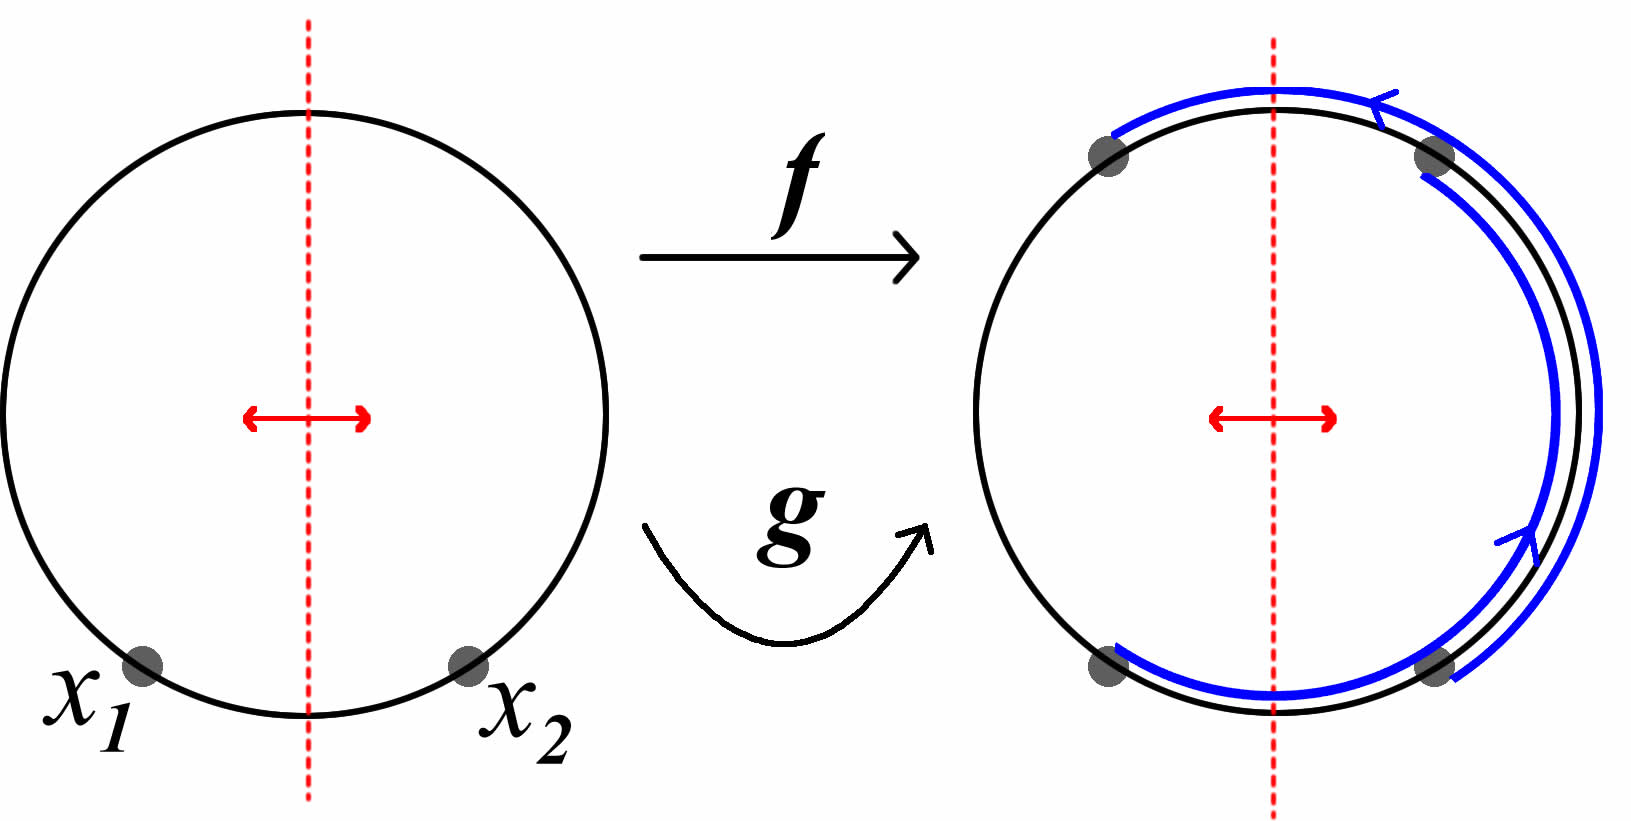
\includegraphics[scale=0.12]{Images/NonEquivariantHomotopyPrism.jpg}
\label{fig:NonEquivariantHomotopyPrism}
\caption{Prism from non-equivariant homotopy}
\end{minipage}
\end{figure}
\end{example}

If we were to use the tools developed in later sections, we would see that \begin{center}$H_n^{alt}(X)=H_n^{alt}(Y)\cong\begin{cases}\mathbb{Z} & n\!=\!1\\0 & n\!\neq\!1\end{cases} \quad$ and that $\quad f_*=1,\,g_*=-1\quad$ (when they're not $0$)\end{center}
So not only would the proof of \ref{EquivariantHomotopyHomomorphism} not work in this case, this is in fact a counter example to the statement for maps that are merely homotopic. It is not, however, a counter example to corollary \ref{Cor:SkHomotopyEquivalence} if the equivariant condition on the homotopy were dropped there too.

\vspace{2mm}
\begin{example}
\label{ex:AltHomOfDiscIsTrivial}
Let us now use the result to show something useful. Take $X=\triangle^n$ the standard $n$-simplex embedded in $\mathbb{R}^{n\!+\!1}$ as usual, with the action of $S_{n\!+\!1}$ being to permute the coordinates. If $X$ has barycentre $\mathbf{b}=\frac1{n+1}(1,\dots,1)$, define $f\!:\!X\!\longrightarrow\!\{\mathbf{b}\}$ to be the constant map, and $g\!:\!\{\mathbf{b}\}\!\longrightarrow\!X$ to be the identity on $\{\mathbf{b}\}$. See $fg=\mathbb{1}_{\{\mathbf{b}\}}$. Take $F$ to be the radial contraction of the simplex to $\mathbf{b}$.
$$F\!:\!X\!\times\!I\!\longrightarrow\!\mathbb{R}^{n\!+\!1} \quad F(\mathbf{x},t)=(t-1)\mathbf{x} + t\mathbf{b}$$
$\mathbf{b}$ is fixed by any $\sigma\in S_{n\!+\!1}$, so we have $\sigma(F(\mathbf{x},t))=(t\!-\!1)\sigma(\mathbf{x})\!+\!t\sigma(\mathbf{b})=F(\sigma(\mathbf{x}),t)$. Hence $F$ is an $S_{n\!+\!1}$-homotopy from $\mathbb{1}_X$ to $gf$, and thus we have show $X$ is $S_{n\!+\!1}$-homotopic to a point. By $S_{n\!+\!1}$-homotopy invariance of singular alternating homology, and example \ref{onePointSpace}, we now have
$$H_k^{alt}(\triangle^n)=0\quad \forall k,n$$
Indeed any space that is $S_k$-contractible to a point (i.e. there is an equivariant contraction) will have trivial alternating homology.
\end{example}

\subsection{Relative Alternating Homology}
\label{Sec_AlternatingRelativeHomology}
\begin{defn}
If $A\subset X$ are both $S_k$-spaces, then $A$ is an \emph{$S_k$-subspace} of $X$ if the action on $A$ is a restriction of the action on $X$.
\end{defn}
\begin{defn}
Given $S_k$-space $X$ and $S_k$-subspace $A$, we define the \emph{Relative Alternating Chain Groups}
$$C_n^{alt}(X,A)\coloneqq\frac{C_n^{alt}(X)}{C_n^{alt}(A)}$$
Using the ordinary boundary map we construct chain complex
$$\dots\longrightarrow C_3^{alt}(X,A)\overset\partial\longrightarrow C_2^{alt}(X,A)\overset\partial\longrightarrow C_1^{alt}(X,A)\overset\partial\longrightarrow C_0^{alt}(X,A)\longrightarrow 0$$
and so we may define the \emph{Relative Alternating Homology Groups} ${H_n^{alt}(X,A)}$ to be the homology groups of this complex.
\end{defn}
A \emph{Relative Alternating Cycle} is an $\alpha\in C_n^{alt}(X)$ such that $\partial\alpha\in C_{n\!-\!1}^{alt}(A)$, and $[\alpha]\in H_n^{alt}(X,A)$ is trivial iff $\alpha = \partial\beta\!+\!\gamma$ for some $\beta\in C_{n\!+\!1}^{alt}(X)$ and $\gamma\in C_n^{alt}(A)$.

\vspace{2mm}
\begin{lemma}
\label{lem:LongExactSeqAltRelHom}
The relative alternating homology groups $H_n(X,A)$ fit into the usual long exact sequence
$$\dots\!\overset\partial\longrightarrow\! H_n^{alt}(A)\!\overset i\longrightarrow\! H_n^{alt}(X)\!\overset j\longrightarrow\! H_n^{alt}(X,A)\!\overset\partial\longrightarrow\! H_{n\!-\!1}^{alt}(A)\!\overset i\longrightarrow\! H_{n\!-\!1}^{alt}(X)\!\overset j\longrightarrow\!\dots\!\overset j\longrightarrow\! H_0^{alt}(X,A)\!\longrightarrow\!0$$
\end{lemma}
\begin{proof}
Consider the short exact sequence of chain complexes

\begin{center}
\begin{tabular}{ c c c c c c c c c }
    &   & $0\quad$ &   & $0\quad$ &   & $0\quad$ &   &    \\
    &   & $\downarrow\quad$ && $\downarrow\quad$ && $\downarrow\quad$ &&\\
$\dots$ & $\overset\partial\longrightarrow$ & $C_{n\!+\!1}^{alt}(A)$ & $\overset\partial\longrightarrow$ &  $C_{n}^{alt}(A)$ & $\overset\partial\longrightarrow$ & $C_{n\!-\!1}^{alt}(A)$& $\overset\partial\longrightarrow$ & $\dots$\\
&   & $\downarrow i$ && $\downarrow i$ && $\downarrow i$ &&\\
$\dots$ & $\overset\partial\longrightarrow$ & $C_{n\!+\!1}^{alt}(X)$ & $\overset\partial\longrightarrow$ &  $C_{n}^{alt}(X)$ & $\overset\partial\longrightarrow$ & $C_{n\!-\!1}^{alt}(X)$& $\overset\partial\longrightarrow$ & $\dots$\\
    &   & $\downarrow j$ && $\downarrow j$ && $\downarrow j$ &&\\
$\dots$ & $\overset\partial\longrightarrow$ & $C_{n\!+\!1}^{alt}(X,A)$ & $\overset\partial\longrightarrow$ &  $C_{n}^{alt}(X,A)$ & $\overset\partial\longrightarrow$ & $C_{n\!-\!1}^{alt}(X,A)$& $\overset\partial\longrightarrow$ & $\dots$\\
    &   & $\downarrow\quad$ && $\downarrow\quad$ && $\downarrow\quad$ &&\\
        &   & $0\quad$ &   &$0\quad$ &   & $0\quad$ &   &    
\end{tabular}
\end{center}
where $i$ is inclusion and $j$ is the map quotienting out by $C_\bullet^{alt}(A)$.

To define $\partial\!:\!H_n^{alt}(X,A)\!\longrightarrow\!H_{n\!-\!1}^{alt}(A)$, take some cycle $c\in C_n^{alt}(X,A)$. By exactness $j$ is surjective, so $\exists\,x\in C_n^{alt}(X)$ such that $j(x)\!=\!c$. Next $\partial x\in C_{n\!-\!1}^{alt}(X)$ is in $\Ker(j)$ since $j(\partial x)=\partial j(x)=\partial c=0$. Hence $\exists\,a\in C_{n\!-\!1}^{alt}(A)$ such that $i(a)=\partial x$. We have that $a$ is a cycle from $i(\partial a)=\partial i(a)=\partial\partial x=0$ and $i$ is injective. Thus we may define $\partial\!:\!H_n^{alt}(X,A)\!\longrightarrow\!H_{n\!-\!1}^{alt}(A)$ by $\partial[c]=[a]$.

By arguments identical to the ordinary relative homology case $\partial$ is well defined, and the sequence it strings these complexes out into is exact via some diagram chasing. The precise details are laid out on page 116 of \cite{algebraictopology}.
\end{proof}

\begin{example}
\label{ex:DiscRelBoundaryIsoSphere}
Consider space $X=\triangle^n$ acted on as per usual by $S_{n\!+\!1}$ permuting coordinates of $\mathbb{R}^{n\!+\!1}$, which restricts to an action on subspace $A=\partial X\subset X$, the boundary of $X$. The long exact sequence from lemma \ref{lem:LongExactSeqAltRelHom} gives
$$\dots\!\overset\partial\rightarrow\! H_1^{alt}(\partial X)\!\overset i\rightarrow\! H_1^{alt}(X)\!\overset j\rightarrow\! H_1^{alt}(X,\partial X)\!\overset\partial\rightarrow\! H_{0}^{alt}(\partial X)\!\overset i\rightarrow\! H_{0}^{alt}(X)\!\overset j\rightarrow\! H_0^{alt}(X,\partial X)\!\rightarrow\!0$$
We recall from example \ref{ex:AltHomOfDiscIsTrivial} that $H_k^{alt}(X)\!=\!0$ for all $k$, giving by exactness $H_k^{alt}(X,\partial X)\cong H_{k\!-\!1}^{alt}(\partial X)$. Via an $S_{n\!+\!1}$-homotopy that stretches $X$ out radially into a regular disc and takes its boundary to a regular circle, we can now say
$$H_k^{alt}(D^n,\partial D^n)\cong H_{k\!-\!1}^{alt}(S^{n\!-\!1})\quad \forall\,k$$
Notice that the result in the ordinary case is $H_{k}(D^n,\partial D)\cong \widetilde{H}_{k\!-\!1}(S^{n\!-\!1})$ due to the use of reduced absolute homology groups in the long exact sequence to take into account that  $H_0(X)\cong\mathbb{Z}$. No such adjustment is necessary in alternating homology, and we can start to feel justified in the decision not to create a reduced alternating homology.
\end{example}

\vspace{1mm}
\begin{example}\label{Ex:AltHomRelPt}
It will be useful to consider the alternating homology of any space $X$ relative to a point $x\in X$. For our definition to hold $x$ must be fixed by the action of $S_k$ on $X$. Then we could use the approach of example \ref{ex:DiscRelBoundaryIsoSphere}, inspecting the long exact sequence
$$\dots\!\overset\partial\rightarrow\! H_1^{alt}(\{x\})\!\overset i\rightarrow\! H_1^{alt}(X)\!\overset j\rightarrow\! H_1^{alt}(X,\{x\})\!\overset\partial\rightarrow\! H_{0}^{alt}(\{x\})\!\overset i\rightarrow\! H_{0}^{alt}(X)\!\overset j\rightarrow\! H_0^{alt}(X,\{x\})\!\longrightarrow\!0$$
The alternating homology of the point is trivial in all dimensions, so again without having to pass to reduced homology we see that 
$$H_n^{alt}(X,\{x\})\cong H_n^{alt}(X)\quad\forall\,n$$
However this argument is really a lot of superfluous machinery. The alternating chain groups of a point are all trivial, so looking directly at the alternating relative chain groups, $C_\bullet^{alt}(X,\{x\})=C_\bullet^{alt}(X)$ and the result falls out very naturally.
\end{example}\vspace{2mm}

\begin{remark}
As in the ordinary case, the proof of \ref{lem:LongExactSeqAltRelHom} can be generalised to associate a long exact sequence to the short exact sequence of chain complexes 
$$0\longrightarrow C_n^{alt}(A,B)\overset{i}\longrightarrow C_n^{alt}(X,B)\overset{j}\longrightarrow C_n^{alt}(X,A)\longrightarrow 0$$
where $B\subset A\subset X$ are $S_k$-spaces/subspaces, $i$ is inclusion into $X$ and $j$ is a quotient by chains in $A$. This gives us the long exact sequence of the triple $(X,A,B)$,
$$\dots\!\rightarrow H_n^{alt}(A,B)\!\rightarrow\!H_n^{alt}(X,B)\!\rightarrow\!H_n^{alt}(X,A)\!\rightarrow\!H_{n\!-\!1}^{alt}(A,B)\!\rightarrow\!H_{n\!-\!1}^{alt}(X,B)\!\rightarrow\!H_{n\!-\!1}^{alt}(X,A)\!\rightarrow\dots$$
\end{remark}



\subsection{Excision}
\label{Sec:Excision}
An important result in ordinary homology is Excision, which describes when the relative homology groups $H_n(X,A)$ are unaffected by removing some subset of $A$. We will mirror Hatcher's proof of this to get the same statement in alternating homology.

In the proof of theorem \ref{EquivariantHomotopyHomomorphism} we referred to the prism operator as a chain homotopy. A proper definition is given here.

\begin{defn}
Any chain maps $f,g\!:\!C_n^{alt}(X)\!\longrightarrow\!C_n^{alt}(Y)$ for which there exists operator $P\!:\!C_n^{alt}(X)\!\longrightarrow\!C_{n\!+\!1}^{alt}(Y)$ satisfying $\partial P + P\partial = f-g$ are called \emph{Chain Homotopic}, and $P$ is called a \emph{Chain Homotopy}.
\end{defn}

\begin{corollary}\label{Cor:ChnHmtpcChnMps_SmHmmrphsms}
As shown in the last few lines of theorem \ref{EquivariantHomotopyHomomorphism}, chain-homotopic chain maps induce the same homomorphisms on alternating homology groups.
\end{corollary}

\begin{lemma}\label{Lem:SkHomotopicMapsOfPairs}
Suppose $f,g\!:\!(X,A)\!\longrightarrow\!(Y,B)$ are $S_k$-homotopic through maps of pairs $(X,A)\!\rightarrow\!(Y,B)$. That is, the chosen $S_k$-homotopy takes $A$ into $B$ at all stages of the deformation. Then $f_*=g_*\!:\!H_n^{alt}(X,A)\!\longrightarrow\!H_n^{alt}(Y,B)$.
\end{lemma}
\begin{proof}
The prism operator from the proof of theorem \ref{EquivariantHomotopyHomomorphism} constructed with the assumed $S_k$-homotopy through maps of pairs will take $C_n^{alt}(A)$ to $C_{n\!+\!1}^{alt}(B)$. Quotienting out to get relative groups, it will then induce the relative prism operator $P\!:\!C_n^{alt}(X,A)\!\rightarrow\!C_{n\!+\!1}^{alt}(Y,B)$, and the relation $\partial P + P\partial=g_\#-f_\#$ is unaffected. Thus $f_\#$ and $g_\#$ are chain homotopic on relative chain groups, so by corollary \ref{Cor:ChnHmtpcChnMps_SmHmmrphsms} they induce the same homomorphism on relative alternating homology groups.
\end{proof}

\begin{thm}
Given $S_k$-spaces and $S_k$-subspaces $Z\subset A\subset X$ such that the closure of $Z$ is in the interior of $A$, the inclusion $(X\setminus Z,A\setminus Z)\xhookrightarrow{} (X,A)$ induces isomorphisms $H_n^{alt}(X\setminus Z,A\setminus Z)\longrightarrow H_n^{alt}(X,A)$.
\end{thm}

Defining $B=X\setminus Z$ and seeing that the action of $S_k$ on $X$ will now restrict to an action on $B$, this Excision theorem has an equivalent formulation.

\vspace{2mm}
\begin{thm}
\label{Thm:Excision}
Take $S_k$-subspaces $A,B\subset X$ such that the interiors of $A$ and $B$ cover $X$. Then inclusion $(B,A\cap B)\xhookrightarrow{}(X,A)$ induces isomorphisms $H_n^{alt}(B,A\cap B)\longrightarrow H_n^{alt}(X,A)$.
\end{thm}

To prove these results, we're going to need to formalise the idea that given an open cover of the space (like $\{A,B\}$) we can subdivide any singular simplex into "smaller" ones until each of them fits properly into a set of the cover.

\begin{defn}
Given $S_k$-space $X$ and a set $\mathfrak{U}=\{U_j\}$ of subspaces whose interiors cover $X$ (note this does not mean $S_k$-subspaces), define
$$C_{n,\mathfrak{U}}^{alt}(X)\coloneqq\{\Sigma_in_i\sigma_i\in C_n^{alt}(X) \mid \forall\,\sigma_i,\, \Ima{\sigma_i}\subset \overset\circ U_j \,\text{ for some }\,U_j\in\mathfrak{U}\}$$
where $\overset\circ U_j$ denotes the interior of $U_j$. The normal boundary map preserves this partitioning condition, so we have a chain complex and may denote its homology $H_{n,\mathfrak{U}}^{alt}$(X). These are alternating versions of $C_{n,\mathfrak{U}}(X)$ and $H_{n,\mathfrak{U}}(X)$, which are defined similarly.
\end{defn}

\vspace{2mm}
\begin{thm}
\label{Thm:OpenCoverChainGroups}
For all $n\!\geq\!0$, the inclusion $\mathfrak{i}\!:\!C_{n,\mathfrak{U}}^{alt}(X)\xhookrightarrow{}C_n^{alt}(X)$ is a chain homotopy equivalence, i.e. there is a chain map $\rho\!:\!C_n^{alt}(X)\!\longrightarrow\!C_{n,\mathfrak{U}}^{alt}(X)$ such that $\mathfrak{i}\rho$ and $\rho\mathfrak{i}$ are chain homotopic to the identity. Hence $\mathfrak{i}$ induces isomorphisms $H_{n,\mathfrak{U}}^{alt}(X)\cong H_n^{alt}(X)$.
\end{thm}
\begin{proof}
Hatcher's proof consists of 4 main stages, which are included for completeness. Our only real deviation is on the end of stage $3$ and $4$, where we check the concerned maps take alternating chains to alternating chains.

\emph{Stage 1: Barycentric subdivision.} For simplex $[v_0,\dots,v_n]$, the \textbf{barycentre} is point $b=\Sigma_{i\,=\,0}^{n}\frac1{n\!+\!1}v_i$, the average of all the vertices. The \textbf{barycentric subdivision} of $[v_0,\dots,v_n]$ is inductively defined as the collection of $n$-simplices $[b,w_0,\dots,w_{n\!-\!1}]$, where each $[w_0,\dots,w_{n\!-\!1}]$ is an $(n\!-\!1)$-simplex in the barycentric subdivision of some face $[v_0,\dots,\hat{v}_i,\dots,v_n]$. The process terminates at $0$-simplices, as these are their own barycentre. We want an upper bound on how big a simplex in the subdivision may be. Define the \textbf{diameter} of a simplex to be the greatest distance between any two points of the simplex, using the Euclidean metric inherited from the  $\mathbb{R}^N$ it is embedded in. By convexity this distance will be between two of the vertices. We claim that the diameter of a simplex $[b,w_0,\dots,w_{n\!-\!1}]$ in the subdivision of $[v_0,\dots,v_n]$ is at most $\frac{n}{n\!+\!1}\diam([v_0,\dots,v_n])$, and proceed by induction. The base case $n\!=\!1$ is clear, as a $1$-simplex is divided into two $1$-simplices of exactly $\frac12$ the length/diameter. For general $n\!>\!1$, we can assume the greatest distance in $[b,w_0,\dots,w_{n\!-\!1}]$ is between vertices $b$ and some $w_i$, as if neither vertex concerned is $b$ then the line between them is contained in an $(n\!-\!1)$-simplex from the subdivision and we're done by the inductive assumption.

\begin{minipage}{0.7\textwidth}
Now by construction $w_i=v_j$ for some $j$, so we may define $b_j$ to be the barycentre of $[v_0,\dots,\widehat{v}_j,\dots,v_n]$, meaning the simplex omitting $v_j$. Comparing barycentric coordinates we have that $b=\frac1{n\!+\!1}v_j+\frac n{n\!+\!1}b_j$, lying on the line $[v_j,b_j]$, and the distance $v_j$ to $b$ is $\frac n{n\!+\!1}$ times the length of $[v_j,b_j]$ which is itself in $[v_0,\dots,v_n]$ and hence bounded by $\diam([v_0,\dots,v_n])$. Explicitly,\end{minipage}
\begin{minipage}{0.3\textwidth}
\centering
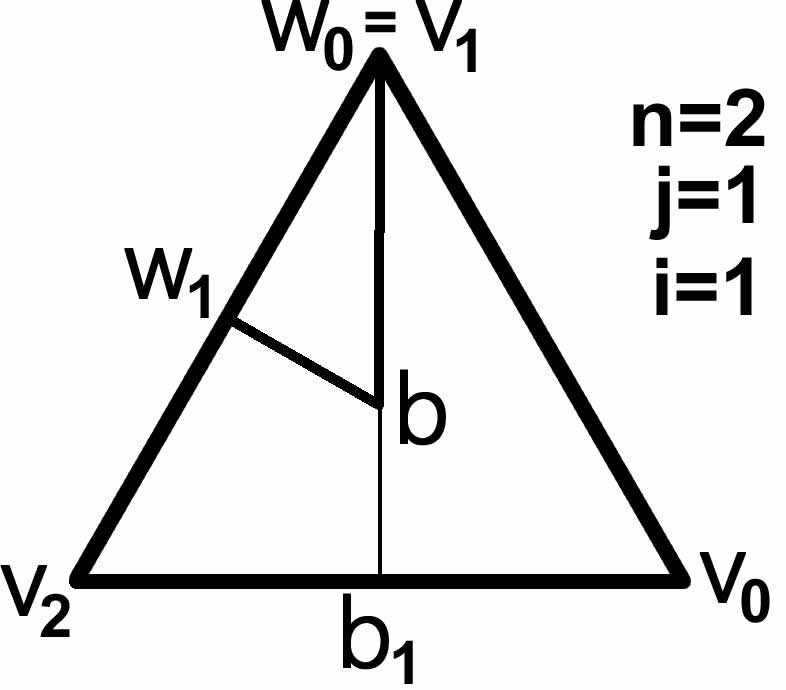
\includegraphics[scale=0.14]{Images/BarycentreOfSubdivision.jpg}
\end{minipage}
$$\diam([b,w_0,\dots,w_n])=\diam([v_j,b])=\frac n{n\!+\!1}\diam([v_j,b_j])\leq \frac n{n\!+\!1}\diam([v_0,\dots,v_n])$$
Our claim is proven, so repeated barycentric subdivision can produce simplices with arbitrarily small diameter.

\emph{Stage 2: Barycentric subdivision of linear chains.}
We aim to construct an operator $S\!:\!C_n^{alt}(X)\!\longrightarrow\!C_n^{alt}(X)$ that subdivides simplices and is chain homotopic to the identity. We start by constructing $S$ on just ordinary 'linear' chains, and later we extend to general ordinary chains before restricting to alternating chains.

For convex set $Y$ in Euclidean space, linear maps $\triangle^n\!\longrightarrow\!Y$ generate a subgroup of $C_n(X)$ which we denote $LC_n(Y)$. The ordinary boundary map takes $LC_n(Y)$ to $LC_{n\!-\!1}(Y)$, so the singular chain complex of $Y$ has a subcomplex of linear chains. A linear map $\lambda\!:\!\triangle^n\!\longrightarrow\!Y$ is uniquely determined by the images $w_i$ of the vertices $v_i$ of $\triangle^n$, so $\lambda$ may be denoted $[w_0,\dots,w_n]$. 

Each point $b\in Y$ determines a homomorphism $b\!:\!LC_n(Y)\!\longrightarrow\!LC_{n\!+\!1}(Y)$ defined on the basis as $b([w_0,\dots,w_n])=[b,w_0,\dots,w_n]$, returning a cone with the $n$-chain as a base and $b$ as the point. Now
$$\partial b([w_0,\dots,w_n])\!=\![w_0,\dots,w_n]\!-\!b(\partial[w_0,\dots,w_n]) \implies \partial b(\alpha)+b(\partial\alpha)\!=\!\alpha\quad\forall\alpha\in LC_n(Y)$$
so $\partial b + b\partial = \mathbb{1}$, i.e. $b$ is an ordinary chain homotopy between the zero map and the identity on $LC_n(Y)$. We are ready to define the subdivision homomorphism $S\!:\!LC_n(Y)\!\longrightarrow\!LC_n(Y)$ by induction on $n$. Take generator $\lambda\in LC_n(Y)$ and define $b_\lambda$ to be the image of the barycentre of $\triangle^n$ under $\lambda$. Then for $n>0$ set $S(\lambda)\coloneqq b_\lambda(S\partial\lambda)$ where $b_\lambda$ is the cone operator above. Letting $S$ be the identity on $LC_0(Y)$, we can see by comparison of definitions that when $\lambda$ is an embedding with image $[w_0,\dots,w_n]$, our choice of $S(\lambda)$ is a signed sum of the simplices in the barycentric subdivision of $[w_0,\dots,w_n]$.

We show inductively that $S$ is a chain map from chain complex $LC_\bullet(Y)$ to itself, i.e. $\partial S=S\partial$. This is trivial in dimension $0$ where $S\!=\!\mathbb{1}$. For $n>1$
\begin{alignat*}{3}
\partial S\lambda & = \partial b_\lambda(S\partial\lambda)\\
& = S\partial\lambda -  b_\lambda\partial (S\partial\lambda) \quad &\text{since }& \, \partial b_\lambda=\mathbb{1}-b_\lambda\partial \\
&=S\partial\lambda-b_\lambda S(\partial\partial\lambda) \quad & \text{since }&\, \partial S(\partial\lambda)=S\partial(\partial\lambda)  & \text{ by inductive assumption}\\
&=S\partial\lambda \quad & \text{since }& \, \partial\partial=0 
\end{alignat*}
Next we want to show $S$ is chain homotopic to the identity on $LC_n(Y)$ by constructing chain homotopy $T\!:\!LC_n(Y)\!\longrightarrow LC_{n\!+\!1}(Y)$, again via an inductive definition. In dimension $0$ define $T([w_0])=[w_0,w_0]$, the constant $1$-simplex. For $n>0$, let $T(\lambda)\coloneqq b_\lambda(\lambda-T\partial\lambda)$. We can visualise the prism $\triangle^n\times I$ divided into simplices, with bottom face $\triangle$ and top face the barycentric subdivision of $\triangle^n$. $T$ takes the image under $\lambda$ of this division after projection through $\triangle^n\times I\longrightarrow\triangle^n$.

In dimension $0$ this is easily seen to be a chain homotopy from $\mathbb{1}$ to $S$, as $\partial T([w_0])+T\partial([w_0])=\partial([w_0,w_0])+0=[w_0]-[w_0]=\mathbb{1}([w_0])+S([w_0])$. For the inductive step, when $n>1$
\begin{alignat*}{4}
\partial T\lambda & = \partial b_\lambda(\lambda-T\partial\lambda)\\
&=\lambda-T\partial\lambda-b_\lambda\partial(\lambda-T\partial\lambda) \quad & \text{ since } & \partial b_\lambda=\mathbb{1}-b_\lambda\partial \\
&=\lambda-T\partial\lambda-b_\lambda(\partial\lambda-\partial T(\partial\lambda))\\
&=\lambda-T\partial\lambda-b_\lambda(S(\partial\lambda)+T\partial(\partial\lambda))\quad & \text{ since } & \mathbb{1}-\partial T=S+T\partial \text{ by inductive assumption }\\
&=\lambda-T\partial\lambda-S\lambda\quad & \text{ since } & \partial\partial=0\,\text{ and } \,b_\lambda(S\partial\lambda)=S\lambda\,\text{ by definition }
\end{alignat*}

\emph{Stage 3: Subdividing general chains.}
We're now able to define $S\!:\!C_n(X)\!\longrightarrow\!C_n(X)$ on singular $\sigma\!:\!\triangle^n\!\longrightarrow X$ by $S(\sigma)\coloneqq\sigma_\#S\triangle^n$, the signed sum of the restrictions of $\sigma$ to each of the simplices in the subdivision of $\triangle^n$. This is still a chain map as, if $\triangle_i^n$ denotes the $i^{th}$ face of $\triangle^n$,
\begin{alignat*}{2}
\partial S\sigma &= \partial\sigma_\#S\triangle^n=\sigma_\#\partial S\triangle^n=\sigma_\#S\partial\triangle^n \\
&= \sigma_\# S(\Sigma_i(-1)^i\triangle_i^n)=\Sigma_i(-1)^i\sigma_\#S\triangle_i^n=\Sigma_i(-1)^iS(\sigma\!\mid_{\triangle_i^n})\\
&=S(\Sigma_i(-1)^i\sigma\!\mid_{\triangle_i^n}) = S(\partial\sigma)
\end{alignat*}
We can similarly extend $T$ to general chains by $T\sigma=\sigma_\#T\triangle^n$, so we still have a chain homotopy between $S\!:\!C_n(X)\!\longrightarrow\!C_n(X)$ and $\mathbb{1}_{C_n(X)}$ by
$$\partial T\sigma\!=\!\partial\sigma_\# T\triangle^n\!=\!\sigma_\#\partial T\triangle^n\!=\!\sigma_\#(\triangle^n\!-\!S\triangle^n\!-\!T\partial\triangle^n)\!=\!\sigma\!-\!S\sigma\!-\!\sigma_\#T\partial\triangle^n\!=\!\sigma\!-\!S\sigma\!-\!T(\partial\sigma)$$
The last equality is by an identical argument to the above proof of the same property for $S$. 

It is time to check that maps $S$ and $T$ restrict usefully to alternating chains. Take $\tau$ in $S_k$ acting on $X$, then $T\sigma\in C_{n\!+\!1}^{alt}(X)$, and $S\sigma\in C_n^{alt}(X)$ for any $\sigma\in C_n^{alt}(X)$, by
\begin{center}$\tau(S\sigma)=\tau(\sigma_\#S\triangle^n)=\tau(\sigma_\#)S\triangle^n=\sgn(\tau)\sigma_\#S\triangle^n=\sgn(\tau)S\sigma$
$\tau(T\sigma)=\tau(\sigma_\#T\triangle^n)=\tau(\sigma_\#)T\triangle^n=\sgn(\tau)\sigma_\#T\triangle^n=\sgn(\tau)T\sigma$\end{center}

\emph{Stage 4: Iterated Barycentric Subdivision.} 
For use in arbitrary subdivision, we create a chain homotopy between $\mathbb{1}$ and $S^m$ called $D_m\!:\!C_n(X)\longrightarrow\!C_{n\!+\!1}(X)$ given by $D_m\coloneqq\Sigma_{0\leq i<m}TS^i$. It must take alternating chains to alternating chains as both $T$ and $S$ do, and it is the chain homotopy we require as
\begin{center}
$\partial D_m+D_m\partial=\underset{0\leq i<m}\sum(\partial TS^i + TS^i\partial)=\underset{0\leq i<m}\sum(\partial TS^i+T\partial S^i)=\underset{0\leq i<m}\sum(\partial T+T\partial)S^i = \underset{0\leq i<m}\sum(\mathbb{1}-S)S^i=\underset{0\leq i<m}\sum(S^i-S^{i+1})=\mathbb{1}-S^m$
\end{center}
Recall that for any open cover of a compact metric space there exists some $\varepsilon\!>\!0$ called the Lebesgue number, such that any set of diameter less than $\varepsilon$ is in some open set in the cover. Thus for each singular $n$-simplex $\sigma\!:\!\triangle^n\!\longrightarrow\!X$, as we have shown the subdivision operator $S$ produces simplices with diameters scaled by at most $\frac n{n\!+\!1}$, there exists positive integer $m$ such that $S^m(\sigma)\in C_{n,\mathfrak{U}}(X)$, i.e. each simplex can be subdivided into simplices contained properly in sets from $\mathfrak{U}$. Denote the minimum such $m$ for each $\sigma$ by $m(\sigma)$. Then let $D\!:\!C_n(X)\!\longrightarrow\!C_{n\!+\!1}(X)$ be given by $D(\sigma)\coloneqq D_{m(\sigma)}(\sigma)$. This is our final, fully formed chain homotopy. But of what? In a slightly backwards fashion, we reverse engineer the chain map out of $D$, calling it $\rho\!:\!C_n(X)\!\longrightarrow\!C_n(X)$.
$$\rho\coloneqq\mathbb{1}-\partial D - D\partial$$
So $D$ is a chain homotopy from $\mathbb{1}$ to $\rho$, which is a chain map as
$$\partial\rho(\sigma)\!=\!\partial\sigma\!-\!\partial^2D\sigma\!-\!\partial D\partial\sigma\!\quad=\quad\!\partial\sigma\!-\!\partial D\partial\sigma \quad=\quad \partial\sigma\!-\!\partial D\partial\sigma-D\partial^2\sigma\!=\!\rho(\partial\sigma)$$
Our intention is for $\rho$ to take $C_n(X)$ into $C_{n,\mathfrak{U}}(X)$, which we check explicitly.
\begin{alignat*}{3}
 \rho(\sigma)&=\sigma-\partial D\sigma-D(\partial\sigma)=\sigma-\partial D_{m(\sigma)}\sigma-D(\partial\sigma)\\
&=S^{m(\sigma)}\sigma+D_{m(\sigma)}(\partial\sigma)-D(\partial\sigma)  & \quad \text{ since } & \partial D_m+D_m\partial=\mathbb{1}-S^m
\end{alignat*}
The $S^{m(\sigma)}\sigma$ term lies in $C_{n,\mathfrak{U}}(X)$ by our choice of $m(\sigma)$. Now writing $\partial\sigma=\Sigma_jn_j\sigma_j$ for $\sigma_j$ the restriction of $\sigma$ to the $j^{th}$ face of $\triangle^n$, we see that the remaining terms $D_{m(\sigma)}(\partial\sigma)-D(\partial\sigma)$ are linear combinations of terms $D_{m(\sigma)}(\sigma_j)-D_{m(\sigma_j)}(\sigma_j)$. By the way they were chosen $m(\sigma_j)\leq m(\sigma)$ so using the definition of $D_m$ we may write $D_{m(\sigma)}(\sigma_j)-D_{m(\sigma_j)}(\sigma_j)=\Sigma_{i=m(\sigma_j)}^{m(\sigma)}TS^i(\sigma_j)$. Each summand is in $C_{n,\mathfrak{U}}(X)$ since $T$ takes $C_{n\!-\!1,\mathfrak{U}}(X)$ to $C_{n,\mathfrak{U}}(X)$, so we have $\Ima(\rho)\subset C_{n,\mathfrak{U}}(X)$. Additionally, we already know that $S$ and $D_m$ take alternating chains to alternating chains, thus we may restrict  $\rho\!:\!C_{n}^{alt}(X)\!\longrightarrow\!C_{n,\mathfrak{U}}^{alt}(X)$.

Finally, recall from the statement of the theorem the inclusion $\mathfrak{i}\!:\!C_{n,\mathfrak{U}}^{alt}(X)\!\longrightarrow\!C_n^{alt}$, and see
$$\partial D+D\partial=\mathbb{1}-\rho\quad\implies\quad\partial D+D\partial=\mathbb{1}-\mathfrak{i}\rho$$
Hence $\mathfrak{i}\rho$ is chain homotopic to $\mathbb{1}$. Moreover, for all $\sigma\in C_{n,\mathfrak{U}}^{alt}(X)$ we have $m(\sigma)=0$, so $D_{m(\sigma)}(\sigma_j)-D_{m(\sigma_j)}(\sigma_j)=T(\sigma_j)-T(\sigma_j)=0$ for all $j$ in the above argument. This means $\rho(\sigma)=S^0(\sigma)+0=\sigma$ on $C_{n,\mathfrak{U}}^{alt}(X)$, and hence $\rho\mathfrak{i}=\mathbb{1}$.

We have built $\rho$, a chain homotopy inverse for $\mathfrak{i}$, so we are done.
\end{proof}


\textbf{\emph{Proof of \ref{Thm:Excision}}}. \\
Set $\mathfrak{U}=\{A,B\}$, then $C_{n,\mathfrak{U}}^{alt}(X)$ is the group of sums of alternating chains entirely in $A$ or entirely in $B$. In the preceding proof of \ref{Thm:OpenCoverChainGroups} the maps $D,\mathfrak{i},\rho$ and $\partial$ all take chains in $A$ to chains in $A$, so they induce quotient maps when factoring out by $C_n^{alt}(A)$. These quotient maps will also adhere to the relations $\partial D+D\partial=\mathbb{1}-\mathfrak{i}\rho$ and $\rho\mathfrak{i}=\mathbb{1}$, thus isomorphisms on alternating homology are induced by the inclusions $$C_{n,\mathfrak{U}}^{alt}(X)/C_n^{alt}(A)\xhookrightarrow{}C_n^{alt}(X)/C_n^{alt}(A)$$
Additionally, see that $C_n^{alt}(B)/C_n^{alt}(A\cap B)$ and $C_{n,\mathfrak{U}}^{alt}(X)/C_n^{alt}(A)$ are both the free group generated by the alternating singular $n$-simplices in $B$ that do not lie in $A$. Hence,
$$H_n^{alt}(X,A)\cong H_n(\frac{C_{n,\mathfrak{U}}^{alt}(X)}{C_n^{alt}(A)})\cong H_n^{alt}(B,A\cap B)$$ 
\hfill$\blacksquare$


With excision proven we will be able to relate relative alternating homology to absolute alternating homology.

\begin{defn}
For $X$ an $S_k$-space and $A\subset X$ a non-empty closed $S_k$-subspace, we call $(X,A)$ a \emph{Good $\mathbf{S_k}$-Pair} if $A$ is an equivariant deformation retract of some neighbourhood $V$, another $S_k$-subspace of $X$.
\end{defn}

\begin{prop}\label{Prop:GoodSkPairRelativeCongQuotient}
For good $S_k$-pair $(X,A)$, the quotient map $q\!:\!(X,A)\!\longrightarrow\!(X/A,A/A)$ induces isomorphisms $q_*\!:\!H_n^{alt}(X,A)\longrightarrow H_n^{alt}(X/A,A/A)\,\,(\cong H_n^{alt}(X/A)$ by \ref{Ex:AltHomRelPt}$)$.
\end{prop}
\begin{proof}
Let $V$ be the neighbourhood of $A$ as described in the definition of a good $S_k$-pair. We have commutative diagram
\begin{displaymath}
\xymatrix{
    H_n^{alt}(X,A) \ar[r]^{\circled{1}} \ar[d]_{\circled{6}}^{q_*} & H_n^{alt}(X,V) \ar[d]^{q_*} & \ar[l]_{\circled{3}\quad} H_n^{alt}(X\!-\! A,V\!-\! A) \ar[d]_{\circled{5}}^{q_*} \\
    H_n^{alt}(X/A,A/A) \ar[r]^{\circled{2}} & H_n^{alt}(X/A,V/A) & \ar[l]_{\circled{4}\quad\quad} H_n^{alt}(X/A\!-\!A/A,V/A\!-\!A/A)  }
\end{displaymath}
See immediately that maps $\circled{3}$ and $\circled{4}$ are isomorphisms as a good $S_k$-pair satisfies the conditions for excision of $A$. To investigate $\circled{1}$, let $r\!:\!(V,A)\!\longrightarrow\!(A,A)$ be the retraction arising from the equivariant deformation retraction $F$ in the definition of a good $S_k$-pair, and let $\mathfrak{i}\!:\!(A,A)\!\longrightarrow\!(V,A)$ be the inclusion of $A$ into $V$. Both are maps of pairs. $\mathfrak{i}\!\circ\!r=\mathbb{1}_A$ and $r\!\circ\!\mathfrak{i}$ is $S_k$-homotopic to $\mathbb{1}_{V}$ via $F$. Thus by \ref{Lem:SkHomotopicMapsOfPairs}, $H_n^{alt}(V,A)\cong H_n^{alt}(A,A)=0$. Putting this into the long exact sequence of the triple $(X,V,A)$,
$$\dots\!\rightarrow H_n^{alt}(V,A)\!\rightarrow\!H_n^{alt}(X,A)\!\overset{\circled{1}}\rightarrow\!H_n^{alt}(X,V)\!\rightarrow\!H_{n\!-\!1}^{alt}(V,A)\!\rightarrow\!H_{n\!-\!1}^{alt}(X,A)\!\overset{\circled{1}}\rightarrow\!H_{n\!-\!1}^{alt}(X,V)\!\rightarrow\dots$$
we get that $\circled{1}$ is an isomorphism. $F$ induces an equivariant deformation retraction of $V/A$ onto $A/A$, so $\circled{2}$ is also an isomorphism by the same argument. Map $\circled{5}$ which quotients out by $A$ is the identity on the complement of $A$, so induces an isomorphism. Finally, by commutativity of the diagram, we have that map $\circled{6}$ must be an isomorphism, and $A/A$ is a point so as seen in example \ref{Ex:AltHomRelPt} we have
$$H_n^{alt}(X,A)\cong H_n^{alt}(X/A,A/A)\cong H_n^{alt}(X/A)$$
\end{proof}

\begin{remark}
Proposition \ref{Prop:GoodSkPairRelativeCongQuotient} means that for a good $S_k$-pair we may rewrite the long exact sequence of relative alternating homology using only absolute groups.
$$\dots\!\overset\partial\rightarrow\! H_n^{alt}(A)\!\overset i\longrightarrow\! H_n^{alt}(X)\!\overset j\longrightarrow\! H_n^{alt}(X/A)\!\overset\partial\longrightarrow\! H_{n\!-\!1}^{alt}(A)\!\overset i\longrightarrow\! H_{n\!-\!1}^{alt}(X)\!\overset j\rightarrow\!\dots\!\overset j\rightarrow\! H_0^{alt}(X/A)\!\rightarrow\!0$$
\end{remark}

\begin{defn}
If $X$ and $Y$ are $S_k$-spaces, the map $F\!:\!X\longrightarrow Y$ is an \emph{$S_k$-homeomorphism} if it is a continuous equivariant bijection with continuous (equivariant) inverse. Note that, if $G\!:\!Y\longrightarrow X$ is the inverse of $F$, then $F\circ G=\mathbb{1}_Y$ and $G\circ F=\mathbb{1}_X$, so $X$ and $Y$ are $S_k$-homotopy equivalent.
\end{defn}

\vspace{2mm}
\begin{example}\label{Ex:OrbitGenerator} As previously mentioned, the 'nuclear elements' of a space in the context of alternating homology turn out to be orbits of the action. It will therefore be useful to find an explicit generator for the group $H_n^{alt}(Y^n,\partial Y^n)$, where $Y^n\!\coloneqq\!\underset{\sigma\in S_k}{\sqcup}\triangle^n_\sigma$, the disjoint union of $k!$ standard $n$-simplices forming an orbit of $S_k$ with obvious permutation action.
\begin{figure}
\centering
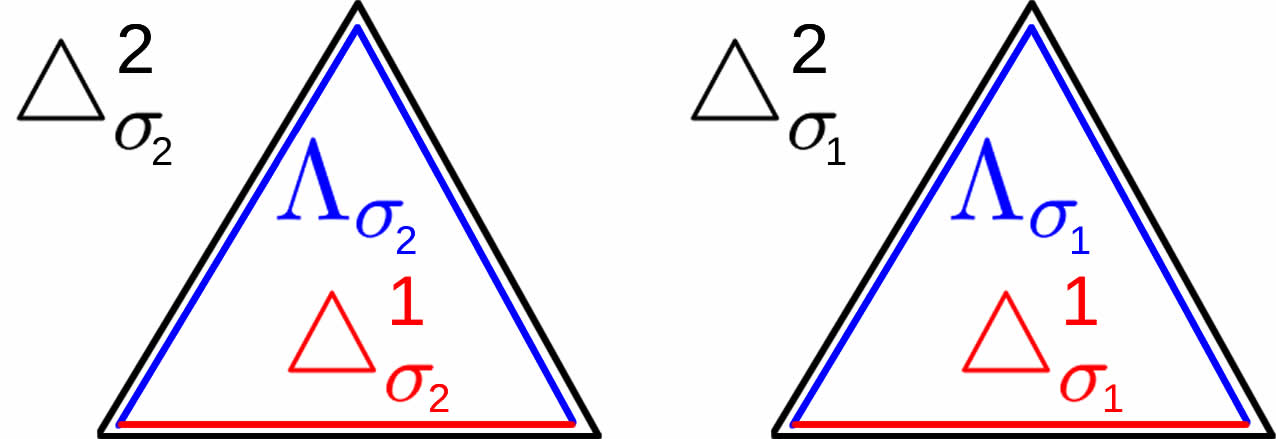
\includegraphics[scale=0.20]{Images/SimplexOrbit.jpg}
\label{fig:SimplexOrbit}
\caption{A disjoint union of simplices forming an orbit of the action of $S_2=\{\sigma_1,\sigma_2\}$}
\end{figure}
We will prove by induction that identity  $\underset{\sigma}\oplus\sgn(\sigma)(id_\sigma\!:\!\triangle_\sigma^n\!\rightarrow\!\triangle_\sigma^n)$ represents such a generator. Firstly it is a cycle, as the boundary in each summand is in $\partial Y^n$. For base case $n=0$ it is clearly a generator, as the chain group of $\partial Y^n$ is empty so it reduces to the general case of example \ref{twoPointSpace}. For the inductive step let each $\Lambda_\sigma\subset\partial\triangle^n_\sigma$ be the union of all but one of the $(n\!-\!1)$-dimensional faces of $\triangle^n_\sigma$ such that we can name the remaining face $\triangle_\sigma^{n\!-\!1}$ and these form an orbit of $S_k$. Figure 8 demonstrates $n=k=2$. Denoting $\Lambda\!\coloneqq\!\underset\sigma\sqcup\,\Lambda_\sigma$ and $Y^{n\!-\!1}\!\coloneqq\!\underset\sigma\sqcup\,\triangle^{n\!-\!1}_\sigma$ we will choose two isomorphisms
$$H_n^{alt}(Y^n,\partial Y^n)\overset{{l}}{\longrightarrow} H_{n-1}^{alt}(\partial Y^n,\Lambda)\overset{{r}}\longleftarrow H_{n-1}^{alt}(Y^{n\!-\!1},\partial Y^{n\!-\!1})$$
The left hand map ${l}$ is found as the boundary map in the long exact sequence of the triple $(Y^n,\partial Y^n,\Lambda )$
$$\dots\longrightarrow H_n^{alt}(Y^n,\Lambda)\longrightarrow H_n^{alt}(Y^n,\partial Y^n)\overset{l}\longrightarrow H_{n\!-\!1}^{alt}(\partial Y^n, \Lambda)\longrightarrow H_{n\!-\!1}^{alt}(Y^n,\Lambda)\longrightarrow\dots$$
For it to be an isomorphism we need $H_n^{alt}(Y^n,\Lambda)\cong 0 \cong H_{n\!-\!1}^{alt}(Y^n,\Lambda)$. Pick any deformation retract $F_1\!:\!\triangle^n_1\times I\!\rightarrow\!\triangle^n_1$ from the simplex $\triangle_1^n$ to $\Lambda_1$, for example figure 9(a), then for each $\sigma\in S_k$ define $F_\sigma\!=\!\sigma F_1(\sigma^{-1}\!\times\!\mathbb{1})$, which moves $F_1$ to the other simplices. This means $\underset\sigma\oplus F_\sigma$ is an equivariant deformation retract from $Y^n$ to $\Lambda$.  Using lemma \ref{Lem:SkHomotopicMapsOfPairs} as before, $H_m^{alt}(Y^n,\Lambda)\cong H_m^{alt}(\Lambda,\Lambda)\cong0$ for all $m\geq0$ and we're done.

The right hand map $r$ follows from proposition \ref{Prop:GoodSkPairRelativeCongQuotient}. Both $(\partial Y^n,\Lambda)$ and $(Y^{n\!-\!1},\partial Y^{n\!-\!1})$ are good $S_k$-pairs, as figure 9(b) and 9(c) demonstrate when $n\!=\!2$. Thus
\begin{figure}
\centering
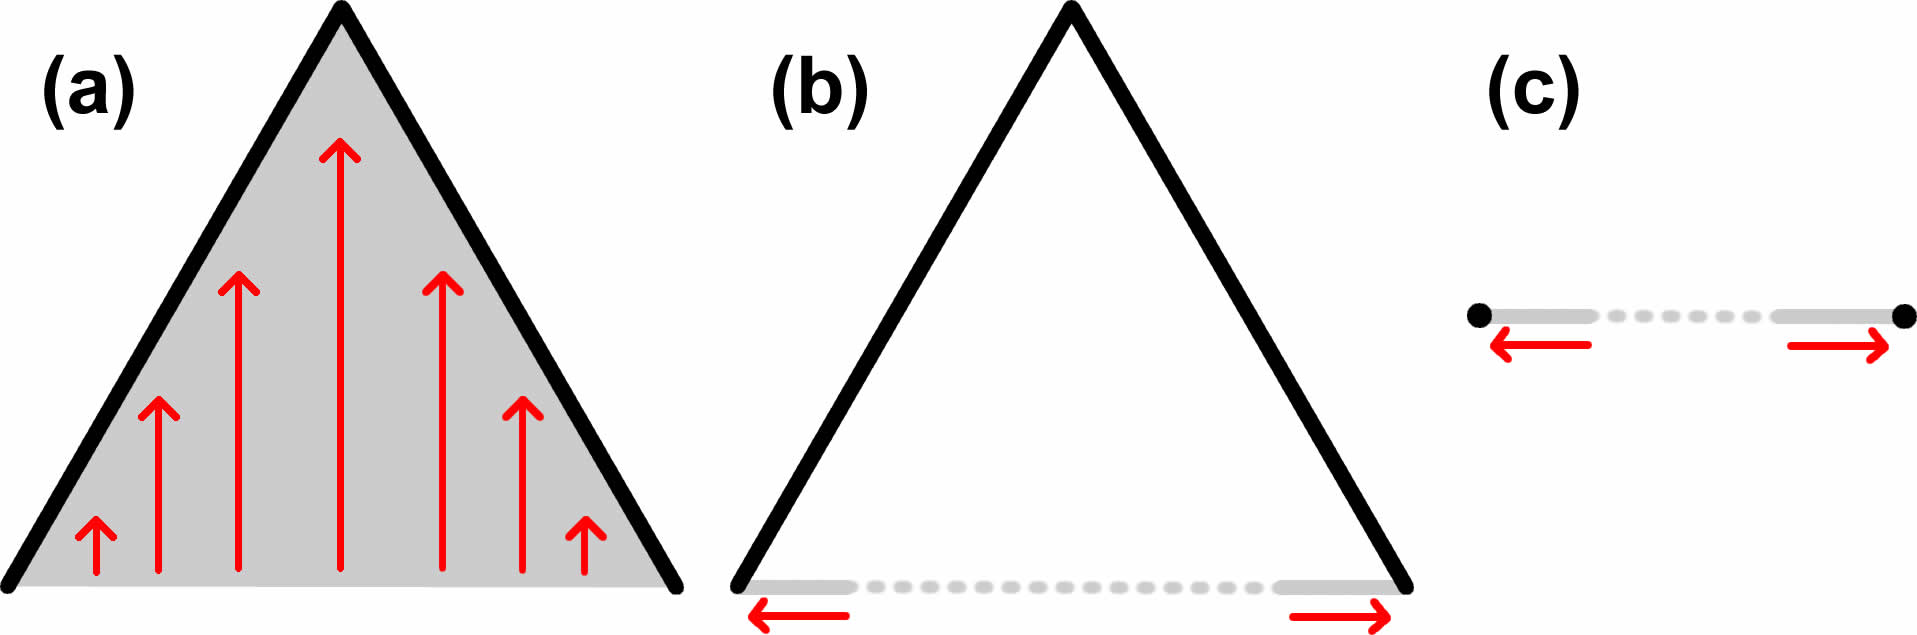
\includegraphics[scale=0.20]{Images/EqDefRetExist.jpg}
\label{Fig:EqDefRetExist}
\caption{Example deformation retracts (showing only one copy of the $n$-simplex in each case). (a) shows $Y^2$ deformation retracting onto $\Lambda$. (b) shows the neighbourhood in $\partial Y^2$ of which $\Lambda$ is a deformation retract. (c) shows the neighbourhood of $\partial Y^1$ in $Y^1$.}
\end{figure}
$$H_{n-1}^{alt}(\partial Y^n, \Lambda)\cong H_{n-1}^{alt}(\partial Y^n / \Lambda)\quad\text{ and }\quad H_{n-1}^{alt}(Y^{n-1},\partial Y^{n-1})\cong H_{n-1}^{alt}(Y^{n-1}/\partial Y^{n-1})$$
The inclusion map $i\!:\!Y^{n\!-\!1}\!\xhookrightarrow\!\partial Y^n$ induces an $S_k$-homeomorphism of the quotient spaces $\partial Y^n/\Lambda \approx Y^{n\!-\!1}/\partial Y^{n\!-\!1}$ so their alternating homology is the same, and hence $H_{n\!-\!1}^{alt}(\partial Y^n,\Lambda)\cong H_{n\!-\!1}^{alt}(Y^{n\!-\!1},\partial Y^{n\!-\!1})$ as required. To complete the inductive step, see that $\underset\sigma\oplus\, id_\sigma$ maps through $l$ to $\underset\sigma\oplus\, \partial\, id_\sigma$ which equals $\pm\underset\sigma\oplus(id_\sigma\!:\!\triangle^{n\!-\!1}_\sigma\!\rightarrow\!\triangle_\sigma^{n\!-\!1})$ in $C_{n\!-\!1}^{alt}(\partial Y^n,\Lambda)$. The inclusion and quotients inducing $r$ preserve this, so
$$H_n^{alt}(Y^n,\partial Y^n)= \langle\underset{\sigma}\oplus(id_\sigma\!:\!\triangle_\sigma^n\!\rightarrow\!\triangle_\sigma^n)\rangle\overset{\pm 1}{\underset\cong\longrightarrow}\langle\underset{\sigma}\oplus(id_\sigma\!:\!\triangle_\sigma^{n-1}\!\rightarrow\!\triangle_\sigma^{n-1})\rangle=H_{n-1}^{alt}(Y^{n-1},\partial Y^{n-1})$$
\end{example}


\begin{example}
\label{Ex:WedgeSumOfOrbits} 
In \ref{Ex:OrbitGenerator} we identified the relative homology of $(Y^n,\partial Y^n)$ with that of the quotient space, a wedge sum of $n$-spheres. It will be useful for theorem \ref{Thm:EquivalenceSimplicialSingular} to extend to the case dealing with multiple orbits.
For fixed $n$ consider $\underset{\alpha}\sqcup Y_\alpha=\underset{\alpha}\sqcup\underset{\sigma\in S_k}\sqcup\triangle^n_{\alpha,\sigma}$, i.e. the disjoint union of multiple orbits, each indexed by $\alpha$ and with corresponding wedge sum $V_\alpha=Y_\alpha/\partial Y_\alpha$. 
The inclusions $i_\alpha\!:\!V_\alpha\xhookrightarrow{}\underset{\alpha}\sqcup V_\alpha$ induce isomorphism $\underset{\alpha}\oplus i_{\alpha *}\!:\!\underset{\alpha}\oplus H_\bullet^{alt}(V_\alpha)\rightarrow H_\bullet^{alt}(\underset{\alpha}\sqcup V_\alpha)$. If $x_\alpha$ is the base point of $V_\alpha$ then the action fixes $\underset{\alpha}\sqcup x_\alpha$, hence the chain groups of this sub-$S_k$-space are all trivial and we take instead the relative homology $\underset{\alpha}\oplus H_\bullet^{alt}(V_\alpha)\cong H_\bullet^{alt}(\underset{\alpha}\sqcup V_\alpha,\underset{\alpha}\sqcup x_\alpha)$. Applying proposition \ref{Prop:GoodSkPairRelativeCongQuotient} gives $\underset{\alpha}\oplus H_\bullet^{alt}(V_\alpha)\cong H_\bullet^{alt}(\underset{\alpha}\vee V_\alpha)$, hence
$$H_\bullet^{alt}(\underset{\alpha}\sqcup Y,\underset{\alpha}\sqcup\partial Y)\cong H_\bullet^{alt}(\underset{\alpha}\sqcup Y/\underset{\alpha}\sqcup\partial Y)\cong H_\bullet^{alt}(\underset{\alpha}\vee V_\alpha) \cong \underset{\alpha}\oplus H_\bullet^{alt}(V_\alpha)\cong \underset{\alpha}\oplus H_\bullet^{alt}(Y_\alpha,\partial Y_\alpha)$$
In particular in dimension $n$ we have $H_n^{alt}(\underset{\alpha}\sqcup Y,\underset{\alpha}\sqcup\partial Y)\cong\underset{\alpha}\oplus \mathbb{Z}$.

This example used possibly more stages than necessary, with the goal of making the correct place to split the group clearer.
\end{example}




\subsection[Simplicial and Singular Equivalence]{Equivalence of Singular and Simplicial Homology}
We are finally ready to equate the singular and simplicial alternating homology groups defined earlier, allowing us to use them interchangeably according to their strengths and weaknesses. Our proof has a similar approach to the ordinary homology case covered in \cite{algebraictopology}, with adaptations to consider properly the orbits of simplices.

\begin{defn}
For $\Delta$-complex $X$, the collection of all simplices in $X$ of dimension $k$ or less is called the $k$-skeleton of $X$.
\end{defn}

\begin{thm}\label{Thm:EquivalenceSimplicialSingular}
Let $S_r$ act simplicially on $\Delta$-complex $X$ and restrict to an action on subcomplex $A\subset X$. The canonical map $\triangle^{alt}_n(X,A)\!\longrightarrow\!C^{alt}_n(X,A)$ which takes each $n$-simplex to its characteristic map $\sigma\!:\!\triangle^n\rightarrow X$ induces an isomorphism $H^{alt}_{n,\triangle}(X,A)\cong H^{alt}_n(X,A)$.
\end{thm}
\begin{proof}
We consider first the case where $X$ is finite dimensional, and $A\!=\!\emptyset$. Denoting the $k$-skeleton of $X$ by $X^k$, the long exact sequence of the pair $(X^k,X^{k-1})$ gives the commutative diagram of sequences
\begin{displaymath}
\xymatrix@C=0.5cm{
    H^{alt}_{n\!+\!1,\triangle}(X^k,X^{k\!-\!1}) \ar[r]^{\,\,\,\partial} \ar[d]^{\circled{1}}   &   H^{alt}_{n,\triangle}(X^{k\!-\!1}) \ar[r]^i \ar[d]^{\circled{2}}  &   H^{alt}_{n,\triangle}(X^k) \ar[r]^{j\quad} \ar[d]^{\circled{3}}   &   H^{alt}_{n,\triangle}(X^k,X^{k\!-\!1}) \ar[r]^\partial \ar[d]^{\circled{4}}   &    H^{alt}_{n\!-\!1,\triangle}(X^{k\!-\!1}) \ar[d]^{\circled{5}}\\
    H^{alt}_{n\!+\!1}(X^k,X^{k\!-\!1}) \ar[r]^{\,\,\,\partial}  &   H^{alt}_{n}(X^{k\!-\!1}) \ar[r]^i   &   H^{alt}_{n}(X^k) \ar[r]^{j\quad}   &   H^{alt}_{n}(X^k,X^{k\!-\!1}) \ar[r]^\partial &  H^{alt}_{n\!-\!1}(X^{k\!-\!1}) 
    }
\end{displaymath}
By the Five Lemma (page 129 of \cite{algebraictopology}), to conclude $\circled{3}$ is an isomorphism it is enough to show that all the other vertical maps are isomorphisms instead. Using an inductive assumption on $k$, $\circled{2}$ and $\circled{5}$ are done for free. The base case $X^0$ is true by means of the argument that follows for the relative homology groups, applied to the pair $(X^0,\emptyset)$.

For $\circled{1}$ and $\circled{4}$, first see the simplicial chain group $\triangle^{alt}_n(X^k,X^{k\!-\!1})$ is $0$ for $n\neq k$. When $n=k$ it is free abelian with basis the alternating chains that are orbits of single $k$-simplices, and $H^{alt}_{n,\triangle}(X^k,X^{k\!-\!1})$ is the same. Next, define map of pairs $\Phi\!:\!(\sqcup_\alpha\triangle^k_\alpha,\sqcup_\alpha\partial\triangle^k_\alpha)\longrightarrow(X^k,X^{k-1})$ using the characteristic maps $\triangle^k\longrightarrow X$ of the simplicial $k$-simplices. We can pull back the action of $S_r$ from $X^k$ via $\Phi$ to a simplicial action on $\sqcup_\alpha\triangle^k_\alpha$, and then split the union up into orbits of this action. $\sqcup_\alpha\triangle_\alpha^k=\sqcup_\beta\sqcup_i\triangle^k_{\beta,i}$, where $i$ indexes the simplices within each orbit $\beta$. Now by example \ref{Ex:WedgeSumOfOrbits} we have $H^{alt}_n(\sqcup_\alpha\triangle_\alpha^k,\sqcup_\alpha\partial\triangle_\alpha^k)\cong \oplus_\beta H^{alt}_n(\sqcup_i\triangle^k_{\beta,i},\sqcup_i\partial\triangle^k_{\beta,i})\cong\oplus_\beta\mathbb{Z}$ generated by the identity on each of the orbits. As we are dealing with good $S_k$-pairs we may consider instead the quotient spaces, wherein $\Phi$ induces an $S_k$-homeomorphism $\sqcup_\alpha\triangle^k_\alpha/\sqcup_\alpha\partial\triangle^k_\alpha\approx X^k/X^{k-1}$. Thus $H_n^{alt}(X^k,X^{k-1})\cong H_n^{alt}(X^k/X^{k-1})$ $\cong \oplus_\beta\mathbb{Z}$, with generators in one-to-one correspondence with the orbits of the characteristic maps $\triangle^k\rightarrow X$. This is the same description as $H^{alt}_{n,\triangle}(X^k,X^{k-1})$, so $\circled{1}$ and $\circled{4}$ are done.

The way we prove the infinite dimensional case is exactly the same as on page 130 of \cite{algebraictopology}. Represent any element of $H_n^{alt}(X)$ by a singular alternating $n$-cycle $z$, which is a linear combination of finitely many singular simplices, each with compact image. $C$, the support of $z$, is therefore compact. Call the interior of a simplex an \emph{open simplex}, and suppose now that $C$ meets infinitely many open simplices in $X$. We may choose a sequence of points $x_i\in C$ each lying in a different open simplex, and can define $U_i=X-\underset{i\neq j}\cup{x_j}$. Each $U_i$ is open as its preimage under the characteristic maps of all the simplices is open, so $\{U_i\}$ is an open cover of $C$ with no finite subcover, contradicting compactness of $C$. Thus we can conclude $C$ meets only finitely many open simplices in $X$, and is contained entirely in $X^k$ for some $k$. Now by our proof of the finite case, $z$ is homologous to a simplicial cycle, and thus as $z$ was arbitrary the map $H_{n,\triangle}^{alt}(X)\rightarrow H_n^{alt}$ is surjective. For injectivity, suppose a simplicial $n$-cycle $z$ is the boundary of a singular $(n\!+\!1)$-chain in $X$. That chain will have compact support again by the previous argument, so will lie in some $X^k$ and hence $z$ is in the kernel of $H_{n,\triangle}^{alt}(X^k)\rightarrow H_n(X^k)$. But this map is injective by the proof of the finite case, so $z$ must be a simplicial boundary in $X^k$ and hence also in $X$.

We now have that $H_{n,\triangle}^{alt}(X)\longrightarrow H_n^{alt}(X)$ is an isomorphism. To prove the case where $A\neq\emptyset$, consider the canonical map between long exact sequences of the pair $(X,A)$.
\begin{displaymath}
\xymatrix@C=0.9cm{
    H^{alt}_{n,\triangle}(A) \ar[r]^{i} \ar[d]  &   H^{alt}_{n,\triangle}(X) \ar[r]^j \ar[d]  &   H^{alt}_{n,\triangle}(X,A) \ar[r]^{\partial} \ar[d]   &   H^{alt}_{n\!-\!1,\triangle}(A) \ar[r]^i \ar[d]   &    H^{alt}_{n\!-\!1,\triangle}(X) \ar[d]\\
    H^{alt}_{n}(A) \ar[r]^{i}  &   H^{alt}_{n}(X) \ar[r]^j   &   H^{alt}_{n}(X,A) \ar[r]^{\partial}   &   H^{alt}_{n\!-\!1}(A) \ar[r]^i &  H^{alt}_{n\!-\!1}(X) 
    }
\end{displaymath}
The four outer maps between absolute groups are isomorphisms by what we have done so far, hence by the Five Lemma the middle map is also an isomorphism.
\end{proof}


\begin{example}
\label{Ex:S3onGenus3Surface}

\begin{figure}
\centering
\begin{minipage}{.48\textwidth}
  \centering
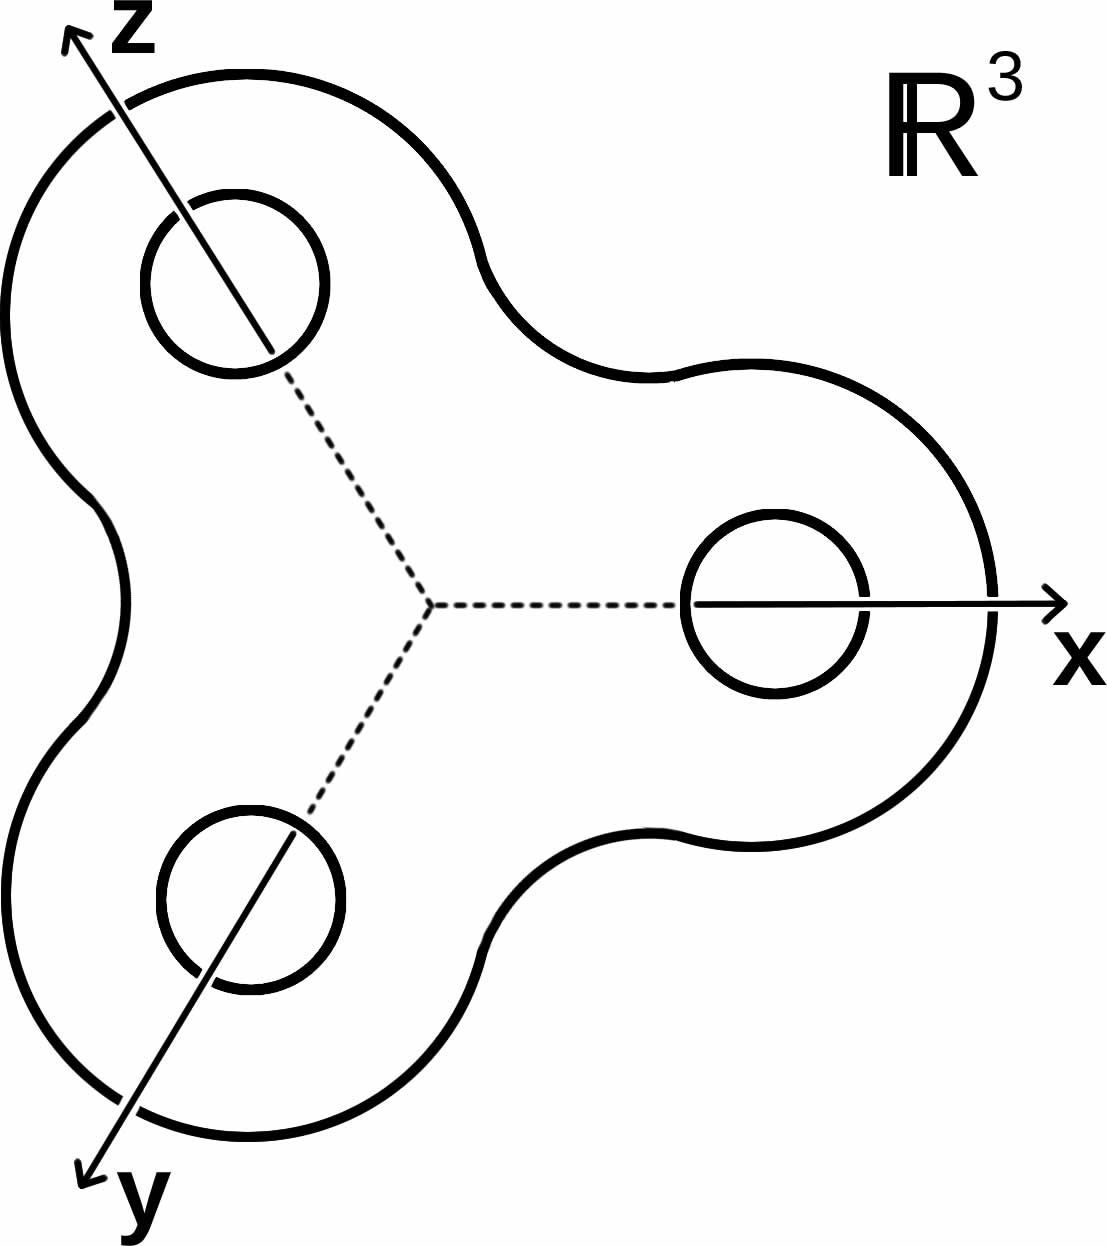
\includegraphics[scale=0.15]{Images/Genus3ActionCrossSection.jpg}
    \vspace{-4mm}
    \caption{The surface of genus $3$, embedded in $R^3$ so as to be "parallel" to the plane $x+y+z=1$. Permutations of coordinates will permute the holes. }
    \label{Fig:S3onGenus3Surface}

\end{minipage}%
\hfill
\begin{minipage}{.48\textwidth}
  \centering
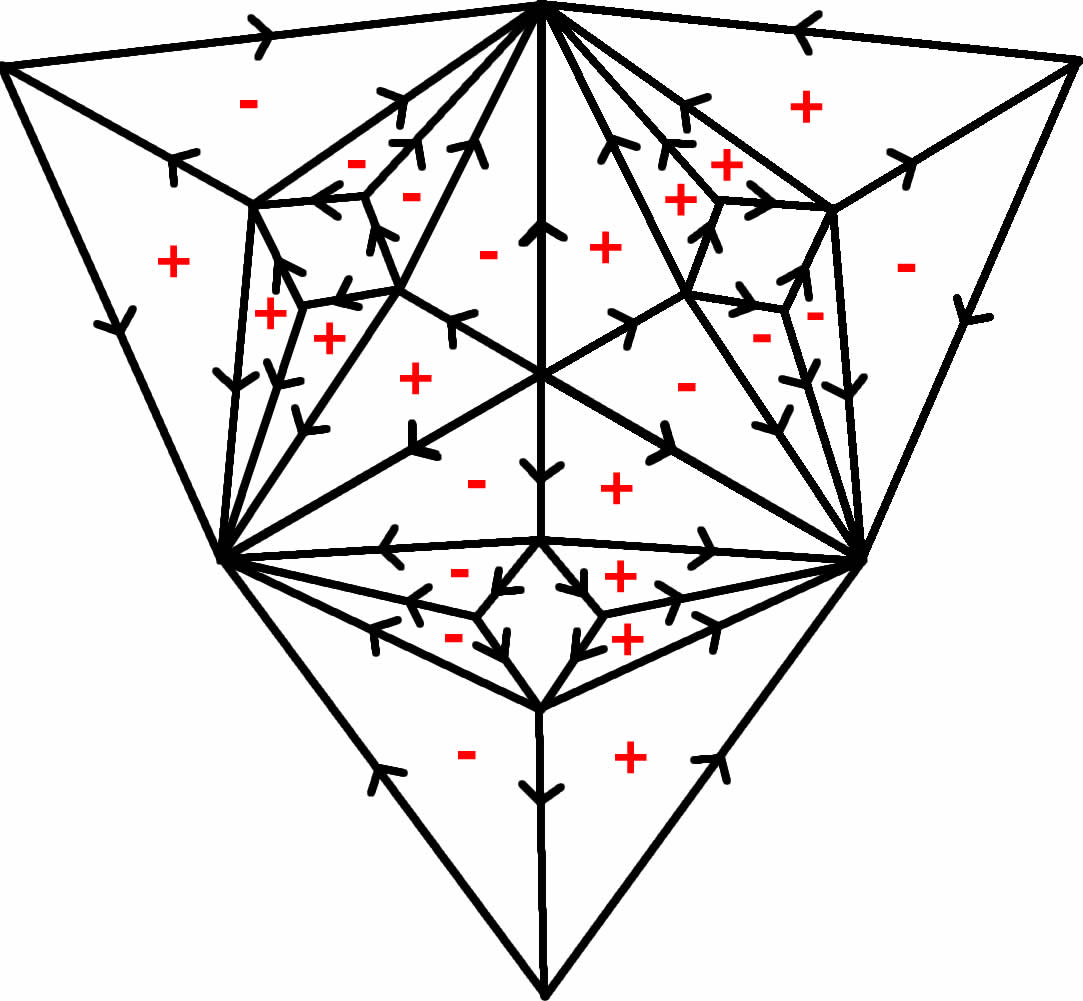
\includegraphics[scale=0.18]{Images/Genus3ActionDeltaComplex.jpg}
\vspace{-4mm}
    \caption{One half (the top) of a $\Delta$-complex for the surface of genus $3$ admiting the action of $S_3$. Signs for $4$ alternating $2$-chains included.}
    \label{Fig:S3onGenus3DeltaComplex}
\end{minipage}


\centering
\begin{minipage}{.48\textwidth}
  \centering
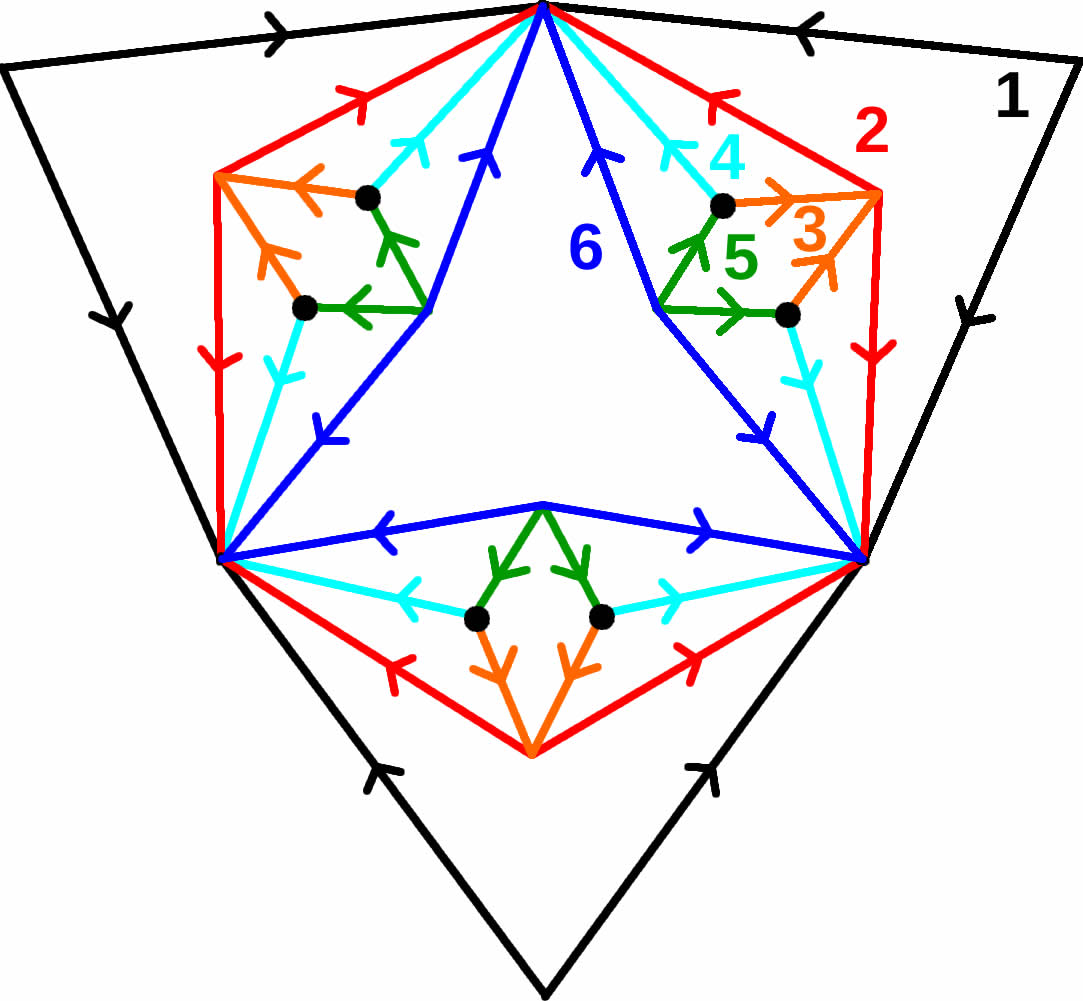
\includegraphics[scale=0.18]{Images/Genus3Alt1Chains.jpg}
    \caption{The alternating $1$-chains of the $\triangle$-complex, labeled for computation. The alternating $0$-chain is also present as black dots.}
    \label{Fig:Genus3Alt1Chains}

\end{minipage}%
\hfill
\begin{minipage}{.48\textwidth}
  \centering
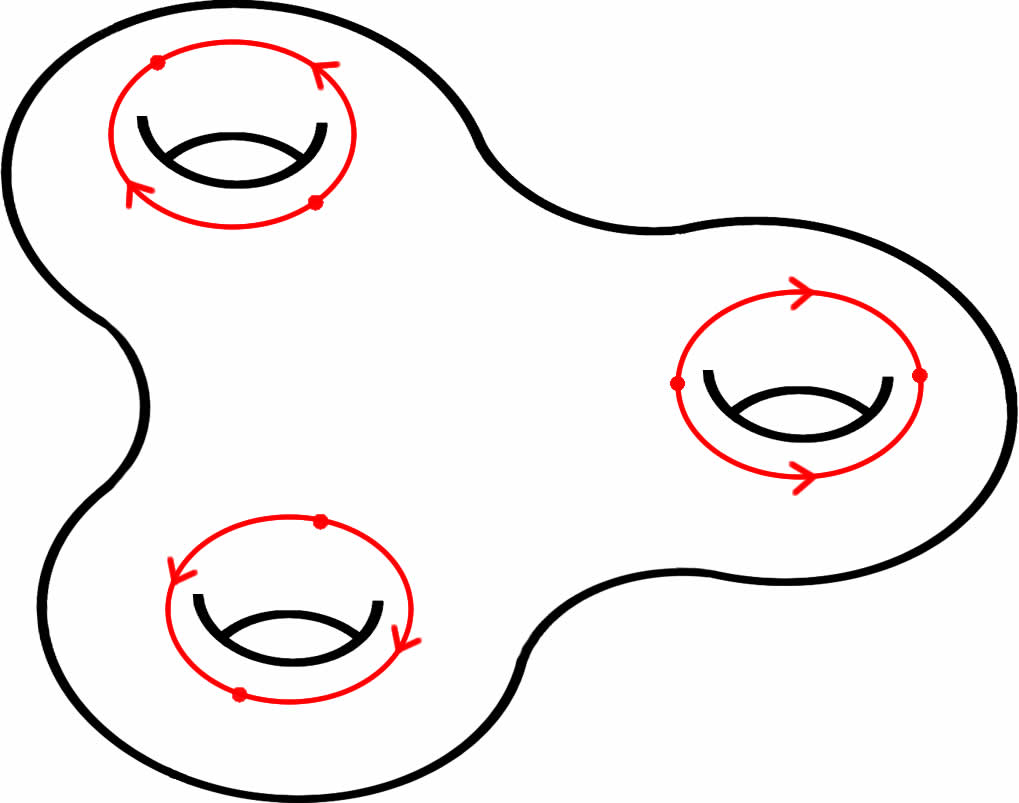
\includegraphics[scale=0.18]{Images/Genus3AltHom1Generator.jpg}
    \caption{The generator of $H_1^{alt}(X)$.}
    \label{Fig:Genus3AltHom1Generator}
\end{minipage}


    \centering
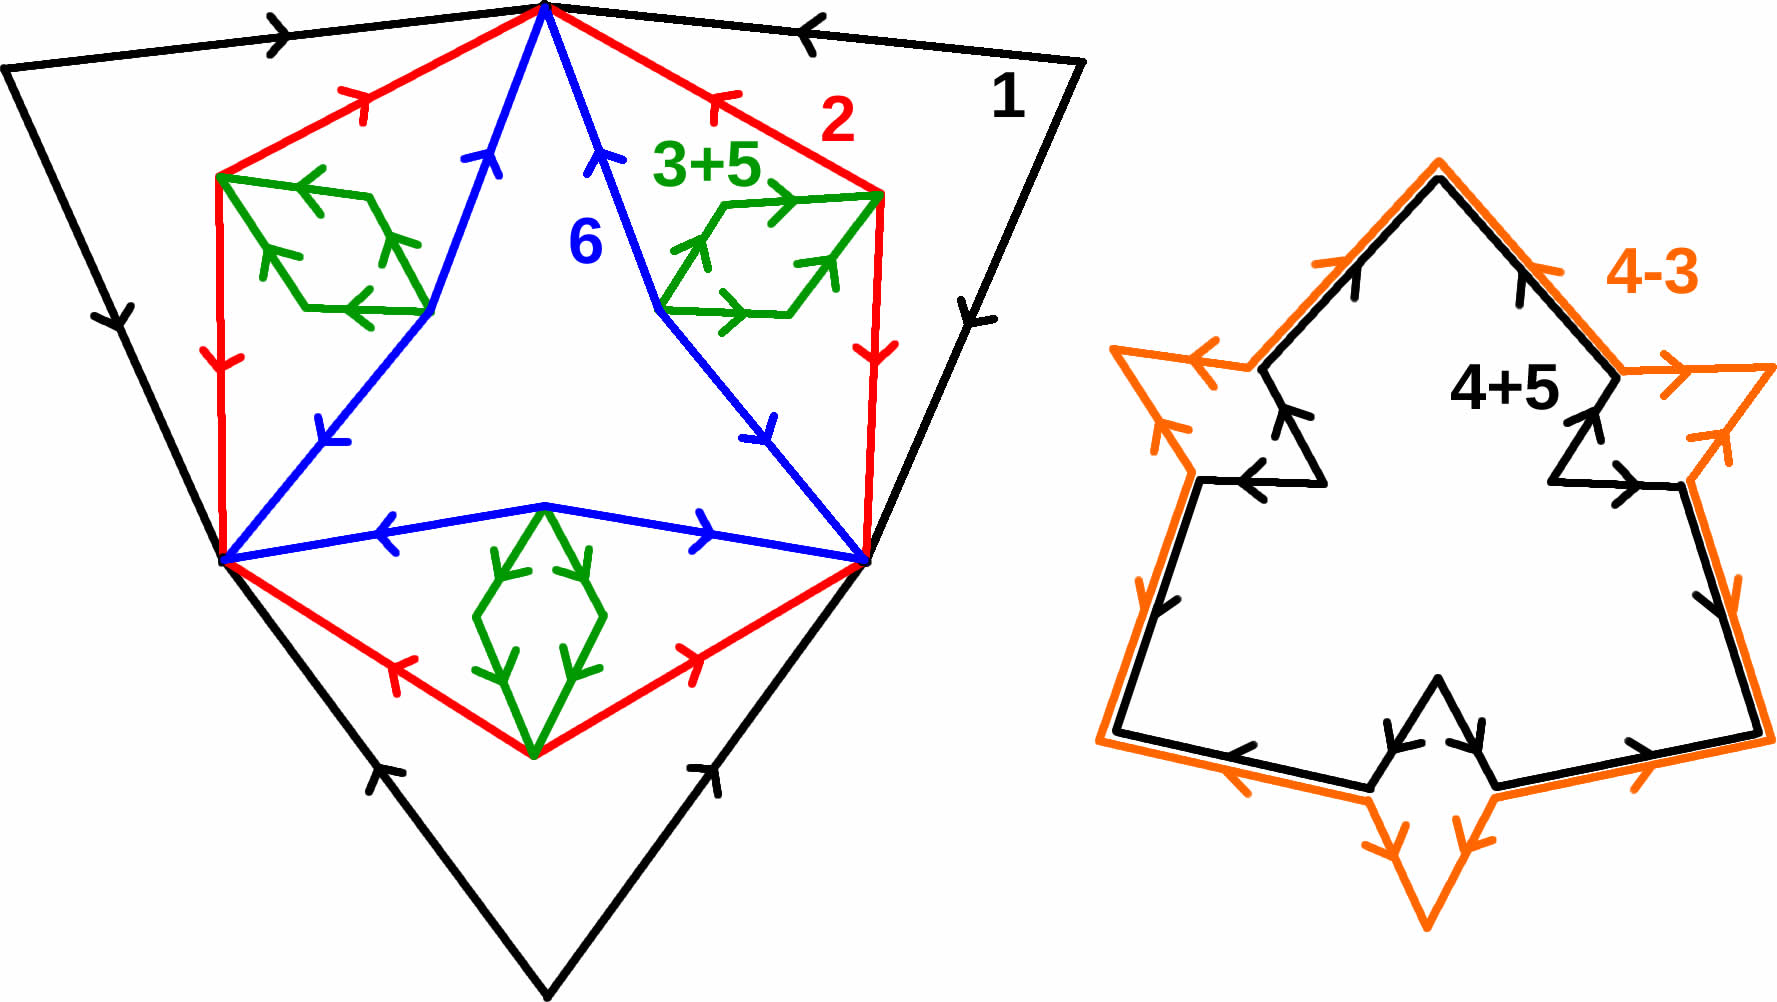
\includegraphics[scale=0.14]{Images/Genus3AltCycles.jpg}
    \caption{The alternating $1$-cycles contained in the top half of the complex. Some are offset to the right for clarity.}
    \label{Fig:Genus3Alt1Cycles}

\end{figure}


We can now compute the singular alternating homology of interesting spaces using the simplicial construction. Let $X$ be the surface of genus $3$, embedded in $\mathbb{R}^3$ with the normal action of $S_3$ permuting copies of $\mathbb{R}$. With the right embedding, the induced action on $X$ could be said to permute the holes using reflections as is obvious in figure \ref{Fig:S3onGenus3Surface}. The $\Delta$-complex $D$ we use is naive and cumbersome, but after calculation it offers a little more clarity about the nature of the generators than more minimalist complexes. Take two copies of the complex shown in figure \ref{Fig:S3onGenus3DeltaComplex} (the second copy using opposite signs) and identify them along their boundary, namely the outer hexagon and the insides of the holes. This space could lie in the plane $\{x+y+z=1\}$, and we see it it would then be $S_k$-homotopic to $X$ via the following two steps. First, stretch the triangular shape to the curved profile of $X$ radially about the line $\{x=y=z\}$, obtaining something still in a plane. Then, pull the top and bottom layers apart along lines perpendicular to $\{x+y+z=1\}$ to fill out into the full form of $X$. Each of these can be defined on one sixth of the shape then mapped through the action to the rest of the space, giving equivariant homotopy equivalences. We have simplicial chain complex
$$0\longrightarrow\triangle_2^{alt}(X)\cong\mathbb{Z}^8\longrightarrow\triangle_1^{alt}(X)\cong\mathbb{Z}^9\longrightarrow\triangle_0^{alt}(X)\cong\mathbb{Z}\longrightarrow0$$
The sum of all alternating $2$-chains is the only $2$-cycle, as all the boundaries cancel by choice of orientations and the opposite signs of the top and bottom half of $D$. The signs of $1$-simplices used to make alternating $1$-chains are numerous and not very interesting, so have been excluded for clarity. The concerned reader can infer them largely from the signs of the $2$-chains and check the following holds. Numbering $1$-chains as in figure \ref{Fig:Genus3Alt1Chains}, the $1$-cycles displayed in part in figure \ref{Fig:Genus3Alt1Cycles} are
$$1,\,2,\,2^\prime,\,6,\,6^\prime,\,3+5,\,4+4^\prime,\,4-3,\,4^\prime+3,\,4+5,\,4^\prime-5$$
where $i^\prime$ denotes the chain corresponding to $i$ on the bottom half of $D$ if it is distinct. See $1-2$, $1-2^\prime$, $1-(4-3)$, and $1-(4^\prime+3)$ are boundaries of alternating chains, so $[1]=[2]=[2^\prime]=[4-3]=[4^\prime+3]$. Obviously $6$, $6^\prime$, $4+5$, and $4^\prime-5$ are boundaries, so they're all trivial in alternating homology. Finally, the boundary of all $2$-simplices in the top half is $1+(3+5)$, so $[1]=-[3+5]$. There is only one alternating $0$-chain, shown in figure \ref{Fig:Genus3Alt1Chains}, and it is the boundary of $3$. Thus we have calculated
$$H_n^{alt}(X)=H_{n,\triangle}^{alt}(D)=\begin{cases} \mathbb{Z} & n=1,2 \\ 0 & n\neq1,2 \end{cases}$$
The ordinary homology of this space is $\mathbb{Z}^6$ in dimension $1$. The alternating part of this ordinary homology group (properly defined in Definition \ref{Def:AltPartHom}) is precisely the alternating homology we just obtained, namely the orbit of the inside of the hole shown in figure \ref{Fig:Genus3AltHom1Generator}. In fact this equivalence is true in all dimensions, but in example \ref{Ex:AntipodalActionOnS1} we will see we cannot expect this to hold for every space.
\end{example}



\subsection{Cellular Alternating Homology}
\label{Sec:CellularAlternatingHomology}
Cellular homology has a natural alternating counterpart which is used in both \cite{Goryunov} and \cite{HoustonTopology}. We again follow Hatcher's construction of ordinary cellular homology to inform our new definition.

\begin{defn}
An $S_k$-space $X$ is an \emph{$S_k$-CW complex} if it is a CW complex such that, for all $n$, $n$-cells are taken to $n$-cells by the free action of $S_k$.
\end{defn}

\begin{remark}
If $X^n$ refers to the $n$-skeleton of $X$, the following two statements are easy observations.
\begin{enumerate}
    \item  When $n\!=\!m$, $H^{alt}_m(X^n,X^{n\!-\!1})$ is free abelian with basis in bijection with the orbits of $n$-cells of $X$. It is trivial for $n\neq m$.
    \item $H^{alt}_m(X^n)=0$ when $m>n$.
\end{enumerate}
The first statement is similar to what we observed in the proof of \ref{Thm:EquivalenceSimplicialSingular}, and follows from the fact that $(X^n,X^{n\!-\!1})$ is a good $S_k$-pair and $X^n/X^{n\!-\!1}$ is a wedge sum of $n$-spheres. For the second, consider part of the long exact sequence of the pair 
$$\dots\longrightarrow H^{alt}_{m+1}(X^n,X^{n-1})\longrightarrow H_m^{alt}(X^{n-1})\longrightarrow H_m^{alt}(X^n)\longrightarrow H_m^{alt}(X^n,X^{n-1})\longrightarrow\dots$$
The two relative groups are trivial by the first statement, so $H^{alt}_m(X^n)\cong H^{alt}_m(X^{n-1})$. Fixing $m$ and letting $n$ decrease, repeating this argument gives
$$H^{alt}_m(X^n)\cong H^{alt}_m(X^{n-1}))\cong \dots \cong H^{alt}_m(X^1)\cong H^{alt}_m(X^0)=0\quad(\text{as }m>0)$$
In particular, if $X$ has finite dimension then $X^{\text{dim}X}=X$, so $H^{alt}_m(X)=0$ for all $m>\text{dim}X$.
\end{remark}

\vspace{2mm}
\begin{lemma}
\label{Lem:CellChainProperties}
If $X$ is an $S_k$-CW complex, then for all $m<n$ the inclusion $i\!:\!X^n\xhookrightarrow{} X$ induces an isomorphism $i_*\!:\!H_m^{alt}(X^n)\longrightarrow H_m^{alt}(X)$.
\end{lemma}
\begin{proof}
If $X$ is finite dimensional, inspecting the same segments of the long exact sequence of pairs from the remark above gives $H^{alt}_m(X^n)\cong H^{alt}_m(X^{n+1})\cong\dots\cong H^{alt}_m(X^{n+r})$ for all $r>0$, as this time $m<n<n+r$. Letting $n+r>\text{dim}X$, we have $H^{alt}_m(X^n)\cong H^{alt}_m(X)$.

For the infinite dimensional case we use a compactness argument similar to that in the proof of \ref{Thm:EquivalenceSimplicialSingular}. An alternating singular chain in $X$ has compact support, so meets only finitely many cells of $X$ and hence lies in a finite skeleton $X^{r}$. Thus an alternating $m$-cycle in $X$ is an alternating cycle in a finite skeleton and by the finite dimensional case it is homologous to an alternating cycle in $X^n$, so we have found a preimage under $i_*\!:\!H^{alt}_m(X^n)\longrightarrow H^{alt}_m(X)$ making it surjective. Similarly if an alternating $m$-cycle in $X^n$ is a boundary of some alternating chain in $X$, then that alternating chain lies in some $X^r$ with $r\geq n$, so by the finite dimensional case the cycle is the boundary of a chain in $X^n$ if $n>m$.
\end{proof}
With this proof done, we may define cellular alternating homology.
Laying out the long exact sequences of the pairs $(X^{n+1},X^n),\,(X^n,X^{n-1})$ and $(X^{n-1},X^{n-2})$ so that they intersect at their shared groups, we get the following diagram.

\begin{center}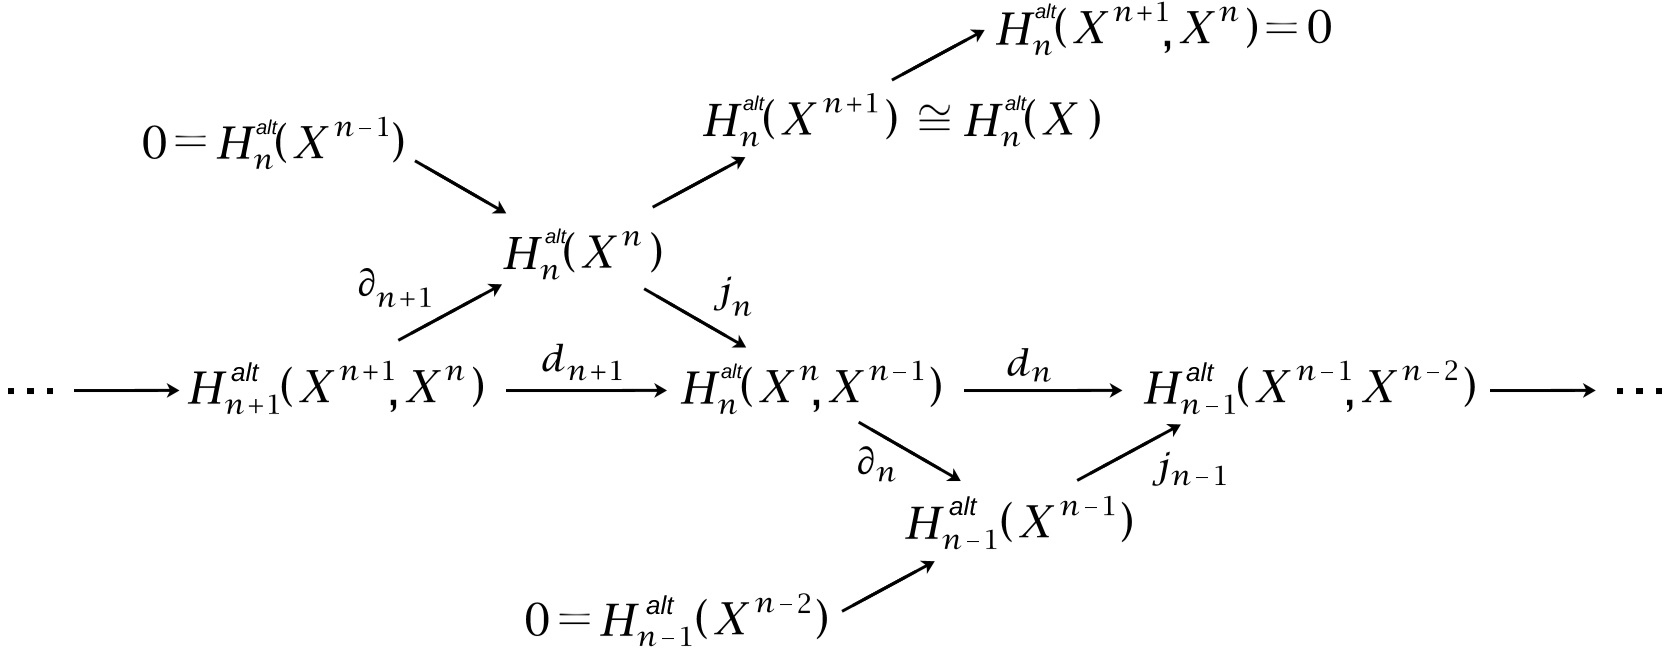
\includegraphics[scale=0.32]{Images/CellularChainComplex.png}\end{center}

The isomorphisms indicated are due to results shown so far in this section. The map $d_n$ is defined to be the composition $j_{n\!-\!1}\partial_n$. The sequence of relative groups with boundary map $d_\bullet$ is a chain complex because $j_n$ and $\partial_n$ are consecutive maps in an exact sequence, meaning $d_nd_{n\!+\!1}=(j_{n\!-\!1}\partial_n)(j_{n}\partial_{n+1})=j_{n\!-\!1}(\partial_nj_{n})\partial_{n+1}=0$.


\begin{defn}
\label{Defn:CellularAlternatingHomology}
The \emph{Cellular Alternating Homology} groups of $S_k$-CW complex $X$ are the homology groups of the cellular alternating chain complex
$$\dots\longrightarrow H^{alt}_{n\!+\!1}(X^{n\!+\!1},X^n) \overset{d_{n+1}}\longrightarrow H^{alt}_{n}(X^n,X^{n\!-\!1}) \overset{d_{n}}\longrightarrow H^{alt}_{n\!-\!1}(X^{n\!-\!1},X^{n\!-\!2})\longrightarrow\dots$$
\end{defn}

\begin{thm}
\label{Thm:EquivalenceCellularSingular}
The cellular alternating homology of a space is isomorphic to the singular alternating homology.
\end{thm}
\begin{proof}
The proof arises easily from inspecting the above diagram. By exactness of the sequence of the pair $(X^{n\!+\!1},X^n)$ we can identify $H^{alt}_n(X)$ with $H^{alt}_n(X^n)/\Ima(\partial_{n\!+\!1})$. If we can get isomorphisms $\Ima(\partial_{n\!+\!1})\cong\Ima (d_{n\!+\!1})$ and $H_n^{alt}(X^n)\cong \Ker (d_n)$ then we will have identified it with $\Ker( d_n)/\Ima( d_{n\!+\!1})$ and be done. Since $j_n$ is injective it gives isomorphism $\Ima(\partial_{n\!+\!1})\cong\Ima(j_n\partial_{n\!+\!1})=\Ima(d_{n\!+\!1})$ so we are half way there. For the next part, again by injectivity of $j_n$, we see $H_n^{alt}(X^n)\cong\Ima(j_n)=\Ker(\partial_n)$. Finally, by the injectivity of $j_{n\!-\!1}$, we have $\Ker(\partial_n)=\Ker (j_{n\!-\!1}\partial_n)=\Ker (d_n)$, so we have shown
$$H^{alt}_n(X)\cong \Ker( d_n)/\Ima( d_{n\!+\!1})$$
\end{proof}

In particular, theorem \ref{Thm:EquivalenceCellularSingular} implies that any two choices of cellular structure compatible with the action of an $S_k$-space will give isomorphic cellular alternating homology. This is a fact that Houston makes implicit use of throughout \cite{HoustonTopology}, so it is reassuring to see it proven.
%Houston makes use of cellular alternating homology in \cite{HoustonTopology}, so through this theorem we can suddenly relate all our preceeding results to 
%\begin{remark}
%In ordinary homology the cellular boundary map $d_n$ can be computed using the cellular boundary formula, $d_n(e^n_\alpha)=\underset\beta\Sigma d_{\alpha\beta} e^{n\!-\!1}_\beta$. Here $e_\alpha^n$ is an $n$-cell identified with a generator of $H_n(X^n,X^{n\!-\!1})$, and $d_{\alpha\beta}$ is the degree of the map $S^{n\!-\!1}_\alpha\rightarrow X^{n\!-\!1} \rightarrow S^{n\!-\!1}_\beta$ given by the composition of the attaching map of $e^n_\alpha$ with the map collapsing $X^{n\!-\!1}-e^{n\!-\!1}_\beta$ to a point.
%\end{remark}

\pagebreak
\setcounter{thm}{0}
\section{Links To Other Theory} \label{Sec:LinksToOtherTheory}
So far we have built a lot of theory from the ground up, and we have developed many useful tools. Now we attempt to relate alternating homology to other areas, in the hope it will add to our understanding or allow us to use better understood theory.

\subsection{Rational Coefficients}\label{Sec:RationalCoefficients}
The following example found in \cite{HoustonSingularityTheory} provides motivation for the use of rational coefficients.

\begin{example}
\label{Ex:AntipodalActionOnS1}
Let $X=S^1$ be acted on by $S_2$, where the non-trivial element $\tau\in S_2$ takes each point to its antipode. This induces an action on the $\Delta$-complex shown in figure \ref{Fig:AntipodalActionOnS1}, formed by identifying the ends of two $1$-simplices head to tail. The ordinary homology is $\mathbb{Z}$ in dimensions $0$ and $1$, generated by $[v_0]$ and $[e_0+e_1]$ respectively. The alternating simplicial chain complex is 
$$0\longrightarrow \triangle_1^{alt}(X)=\langle e_0-e_1\rangle \longrightarrow \triangle_0^{alt}(X)=\langle v_0-v_1\rangle\longrightarrow0$$
where $\partial(e_0-e_1)=2(v_0-v_1)$. This gives $H_1^{alt}(X)=0$ and $H_0^{alt}(X)=\langle [v_0-v_1]\rangle\cong\mathbb{Z}_2$. Notice that $H_0^{alt}(X)$ is not a subgroup of $H_0(X)$, making them difficult to relate. However, if we were working in a context with rational coefficients, $(v_0-v_1)$ would be the boundary of $\frac12(e_0-e_1)$, so the alternating homology group will be a (trivial) subgroup of ordinary homology in every dimension. In general, rational coefficients will get rid of problematic torsion groups. We formalise this with some more definitons.
\begin{figure}[h]
    \centering
    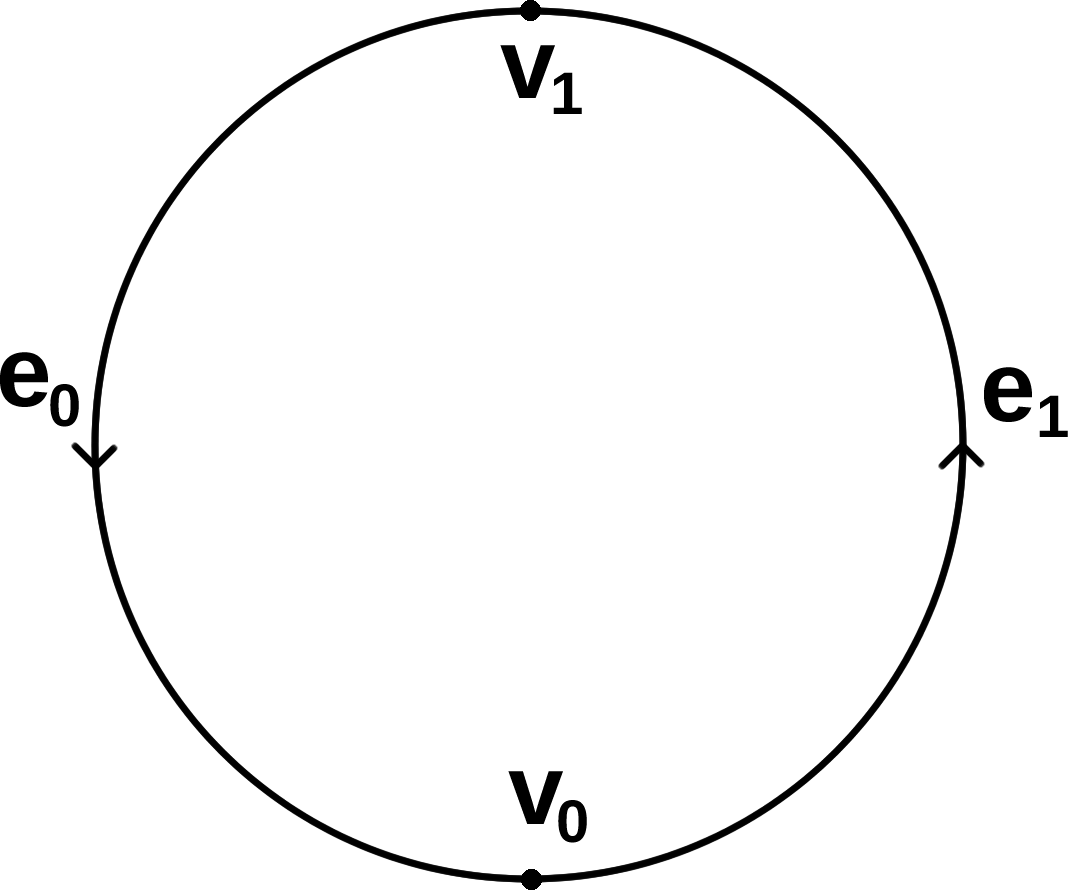
\includegraphics[scale=0.15]{Images/RationalCoeffMotivation.png}
    \caption{A simplicial complex for $S^1$ acted on by $S_2$}
    \label{Fig:AntipodalActionOnS1}
\end{figure}
\end{example}

\begin{defn}\label{Def:HomologyWithCoeff}
For abelian group $G$ and topological space $X$, the chain groups $C_n(X;G)$ are defined as on page 153 in \cite{algebraictopology} as the groups of finite formal sums $\Sigma_in_ic_i$, where each $c_i$ is a singular $n$-simplex and $n_i\in G$. The ordinary boundary map gives a chain complex, so we may define $H_n(X;G)$, the homology of $X$ with coefficients in $G$.
\end{defn}
\begin{defn}\label{Def:AltHomWCoeff}
For $S_k$-space $X$, taking coefficient group $G$ to be $\mathbb{Q}$, we get \emph{Rational Alternating Homology} $H_\bullet^{alt}(X;\mathbb{Q})$ from the chain complex
$$C_n^{alt}(X;\mathbb{Q})\coloneqq\{c_n\in C_n(X;\mathbb{Q})\mid \sigma_\#c_n=\sgn(\sigma)c_n\quad\forall\sigma\in S_k\}$$
\end{defn}

\begin{defn}\label{Def:AltPartHom}
Define the alternating part of the ordinary homology of an $S_k$-space by
\begin{alignat*}{3}
\Alt H_n(X) & \coloneqq \{[c_n]\in H_n(X) \mid \sigma[c_n]=\sgn(\sigma)[c_n]\quad\forall\sigma\in S_k\} \\
&=\{[c_n]\in H_n(X)\mid \forall\sigma\in S_k,\, \exists\, c_{n\!+\!1}^\sigma\in C_{n\!+\!1}(X)\,:\, \sigma_\#c_n\!-\!\sgn(\sigma)c_n\!=\!\partial(c_{n\!+\!1}^\sigma)\}
\end{alignat*}
We extend this definition in the obvious way to $\Alt H_n(X;\mathbb{Q})$.
\end{defn}

The groups defined in \ref{Def:AltHomWCoeff} and \ref{Def:AltPartHom} are the ones we want to relate, chosen because of the existence of the map 
$$A\!:\!C_n(X;\mathbb{Q})\longrightarrow C_n^{alt}(X;\mathbb{Q})\quad\quad A(c_n)\coloneqq\frac1{k!}\Alt=\frac1{k!}\underset{\sigma \in S_k}\sum\sgn(\sigma)\sigma(c_n)$$
\begin{equation}\label{Eq:PreservesAltChains}
c_n\in C^{alt}_n(X;\mathbb{Q})\quad\implies\quad A(c_n)=\frac1{k!}\Sigma_\sigma\sgn(\sigma)\sigma(c_n)\!=\!\frac1{k!}\Sigma_\sigma\sgn^2(\sigma)c_n\!=\!\frac1{k!}k!c_n\!=\!c_n\end{equation}
When working in $\mathbb{Z}$, the $\Alt$ operator would introduce a factor of $k!$. Moving to $\mathbb{Q}$ has allowed us to get rid of this and subsequently preserve alternating chains, enabling our proof of the following lemma.
\\
\begin{lemma}
\label{Lem:EquivAltPartHomQAltHomQ}
The inclusions $\mathfrak{i}\!:\!C_n^{alt}(X;\mathbb{Q})\xhookrightarrow\!C_n(X;\mathbb{Q})$ induce isomorphisms $\Alt H_n(X;\mathbb{Q})\cong H_n^{alt}(X;\mathbb{Q})$.
\end{lemma}
\begin{proof}
The composition $A\mathfrak{i}\!:\!C^{alt}_n(X;\mathbb{Q})\rightarrow C^{alt}_n(X;\mathbb{Q})$ is the identity by (\ref{Eq:PreservesAltChains}) above, and $A$ is clearly a chain map, so these two maps together induce $A_*\mathfrak{i}_*=(A\mathfrak{i})_*=\mathbb{1}_*$. This is an isomorphism, implying in particular that $\mathfrak{i}_*$ is an injective homomorphism. We see that $\Ima(\mathfrak{i}_*)\subset\Alt H_n(X;\mathbb{Q})$, because an alternating chain obeys $\sigma_\#c_n\!-\!\sgn(\sigma)c_n\!=\!\partial(0)$, thus we now need only show that $\mathfrak{i}_*$ is surjective onto $\Alt H_n(X;\mathbb{Q})$.

Take any $[c_n]\in\Alt H_n(X;\mathbb{Q})$, then by rearranging the definition, for all $\sigma\in S_k$ there exists $c_{n\!+\!1}^\sigma\in C_{n\!+\!1}(X)$ such that $\sgn(\sigma)\sigma_\#c_n\!=\!c_n\!+\!\partial(c_{n\!+\!1}^\sigma)$, so
$$ A(c_n)=\frac1{k!}\sum_\sigma\sgn(\sigma)\sigma_\#c_n=\frac1{k!}\sum_\sigma c_n\!+\partial(c_{n\!+\!1}^\sigma)=c_n+\partial(\frac1{k!}\sum_\sigma c_{n\!+\!1}^\sigma)\!=\vcentcolon\!\gamma\in C_n^{alt}(X;\mathbb{Q})$$
This means $\mathfrak{i}(\gamma)-c_n$ is a boundary in $C_n(X;\mathbb{Q})$, hence $\mathfrak{i}_*[\gamma]=[c_n]$ and we're done.
\end{proof}

We have shown how to relate alternating homology to the alternating part of ordinary homology when using rational coefficients, but everything done up until this point has used integers. It would be useful, therefore, to be able to relate rational alternating homology back to integer alternating homology, which is easy enough with a few standard results.

\vspace{2mm}
\begin{defn}
For ring $R$, left $R$-module $N$ and right $R$-module $M$, the tensor product $M\otimes_{R}N$ is defined to be the abelian group generated by the pairs $\{m\otimes n\mid m\in M,\,n\in N\}$ quotiented out by the following relations.
\begin{enumerate}
\item $(m_1+m_2)\otimes n=(m_1\otimes n) + (m_2\otimes n)\quad$ and $\quad m\otimes(n_1+n_2)=(m\otimes n_1) + (m\otimes n_2)$
\item $mr\otimes n=m\otimes rn\quad$ for all $r\in R $
\end{enumerate}
\end{defn}

The following two examples illustrate some easy tensor products, and cover everything we will come across when tensoring homology groups with $\mathbb{Q}$.
\begin{example}\label{Ex:ZtensorQ}
The tensor product $\mathbb{Z}\otimes_\mathbb{Z}\mathbb{Q}$ is isomorphic to $\mathbb{Q}$ via map $\phi\!:\!\mathbb{Z}\otimes_\mathbb{Z}\mathbb{Q}\longrightarrow \mathbb{Q}$ given by $\phi(z\otimes q)=zq$. This is obviously surjective as for any $q\in\mathbb{Q}$ we have $\phi(1\otimes q)=q$. Suppose that $\phi(z_1\otimes q_1)=\phi(z_2\otimes q_2)$, i.e. $z_1q_1=z_2q_2$. Then, using property 2 in the tensor product definition, $z_1\otimes q_1=1\otimes z_1q_1=1\otimes z_2q_2=z_2\otimes q_2$ implying injectivity. Lastly, using both properties, $\phi$ is a homomorphism as
\begin{alignat*}{3}
    \phi(z_1\otimes q_1 + z_2\otimes q_2) & =\phi(1\otimes z_1q_1+1\otimes z_2q_2)\\
    &=\phi(1\otimes(z_1q_1+z_2q_2))=z_1q_1+z_2q_2\\
    &=\phi(z_1\otimes q_1)+\phi(z_2\otimes q_2)
\end{alignat*}
%$$\phi(z_1\otimes q_1 + z_2\otimes q_2)\!=\!\phi(1\otimes z_1q_1+1\otimes z_2q_2)\!=\!\phi(1\otimes(z_1q_1+z_2q_2))\!=\!z_1q_1+z_2q_2\!=\!\phi(z_1\otimes q_1)+\phi(z_2\otimes q_2)$$
\end{example}

\begin{example}
\label{Ex:ZtensorZmodnZ}
It is easy to see that $(\mathbb{Z}/n\mathbb{Z})\otimes_\mathbb{Z}\mathbb{Q}=0$ for any $n>0$. If $z\in\mathbb{Z}/n\mathbb{Z}$ and $q\in\mathbb{Q}$, then $z\otimes q=z\otimes n\frac qn=zn\otimes \frac qn=0\otimes \frac qn$. We see by using property 1 from the definition that $x\otimes \frac qn=(x+0)\otimes \frac qn = (x\otimes \frac qn) + (0\otimes \frac qn)$ for any $x\in\mathbb{Z}/n\mathbb{Z}$, so $0\otimes\frac qn=0$ and hence our arbitrary element $z\otimes q$ is $0$.
\end{example}

We are going to show there exists an isomorphism $H^{alt}_n(X)\otimes_\mathbb{Z}\mathbb{Q}\cong H^{alt}_n(X;\mathbb{Q})$, relating our well-studied integer alternating homology to the construction with rational coefficients. Here $H_n^{alt}(X)$ is treated as a right $\mathbb{Z}$-module in the obvious way, through multiplication of coefficients. The result we use, presented and proved by Chen in \cite{UCT}, is the Universal Coefficient Theorem which reads as follows.

\vspace{2mm}
\begin{thm}\label{Thm:UCT}
If $C$ is a chain complex of free abelian groups, then for any $n\in\mathbb{Z}$ and $G$ a left $\mathbb{Z}$-module there is a short exact sequence
$$ 0\longrightarrow H_n(C)\otimes_\mathbb{Z}G\longrightarrow H_n(C;G)\longrightarrow \Tor(H_{n\!-\!1}(C),G)\longrightarrow 0$$
where $\Tor$ is yet to be defined.
\end{thm}
In particular, letting $C$ be the alternating chain complex of an $S_k$-space $X$, this means 
$$H^{alt}_n(X;\mathbb{Q})\cong (H_n^{alt}(X)\otimes_\mathbb{Z}\mathbb{Q}) \oplus \Tor(H^{alt}_{n\!-\!1}(X),\mathbb{Q})$$
So $\Tor(H^{alt}_{n\!-\!1}(X),\mathbb{Q})$ captures the difference between the two groups we're trying to relate. This theorem is a statement about general chain complexes, so we omit the proof as it is not of special interest for alternating homology. Clearly, however, we must further investigate $\Tor(H^{alt}_{n\!-\!1}(X),\mathbb{Q})$.

\vspace{2mm}
\begin{defn}\label{Def:FreeResolution}
For abelian group $H$, a \emph{Free Resolution} of $H$ is an exact sequence 
$$ \dots\longrightarrow F_2\overset{f_2}\longrightarrow F_1\overset{f_1}\longrightarrow F_0\overset{f_0}\longrightarrow H\longrightarrow 0 $$
where each $F_n$ is free.
\end{defn}
\vspace{2mm}
\begin{defn}
For right $\mathbb{Z}$-module $H$ with a free resolution consisting of right $\mathbb{Z}$-modules $F_i$, we tensor with a left $\mathbb{Z}$-module $Q$ to get a chain complex 
$$\dots\longrightarrow F_2\otimes_\mathbb{Z}Q\xrightarrow{f_2\otimes\mathbb{1}} F_1\otimes_\mathbb{Z}Q\xrightarrow{f_1\otimes\mathbb{1}} F_0\otimes_\mathbb{Z}Q\xrightarrow{f_0\otimes\mathbb{1}} H\otimes_\mathbb{Z}Q\longrightarrow0$$
since $f_nf_{n\!+\!1}\!=\!0$ implies $(f_n\otimes\mathbb{1})(f_{n\!+\!1}\otimes\mathbb{1})\!=\!0$. We then define
$$\Tor(H,Q)\coloneqq\Ker(f_1\otimes\mathbb{1})/\Ima(f_2\otimes\mathbb{1})$$
\end{defn}
For $\Tor$ to be well-defined we require that such a free resolution always exists, and that the choice of free resolution doesn't matter. The first part is easy as Hatcher chooses one explicitly on page 195 of \cite{algebraictopology}. We fix a generating set for the right $\mathbb{Z}$-module $H$, and define $F_0$ to be the free abelian group with basis  $S$ in one-to-one correspondence with these generators. $F_0$ inherits the right $\mathbb{Z}$-action from $H$, and $f_0\!:\!F_0\longrightarrow H$ is a surjective homomorphism taking basis elements in $S$ to their corresponding generators. Next we choose $F_1=\Ker(f_0)$, a subgroup of a free abelian group and hence a free abelian group itself. $f_1\!:\!F_1\longrightarrow F_0$ is an inclusion and therefore injective, so finally we set $F_n=0$ for all $n>1$ to produce the free resolution
$$ \dots\rightarrow 0 \rightarrow 0 \rightarrow \Ker(f_0)\xhookrightarrow{f_1} \langle S\rangle\overset{f_0}\longrightarrow H\longrightarrow 0$$
The invariance of $\Tor$ under different choices of free resolution is lemma 3A.2 in \cite{algebraictopology}, so we may always use the simple one chosen above for computation.

\vspace{2mm}
\begin{lemma}
\label{Lem:Halt(X;Q)congHalt(X)tensorQ}
When $X$ is an $S_k$-space, $\Tor(H^{alt}_{n\!-\!1}(X),\mathbb{Q})=0$ for all $n$, and hence by the Universal Coefficient Theorem $H^{alt}_n(X)\otimes_\mathbb{Z}\mathbb{Q}\cong H^{alt}_n(X;\mathbb{Q})$.
\end{lemma}
\begin{proof}
We are computing $\Ker(f_1\otimes\mathbb1)/\Ima(f_2\otimes\mathbb{1})$ in chain complex
$$ 0\xrightarrow{f_2\otimes\mathbb1}\Ker(f_0)\otimes_\mathbb{Z}\mathbb{Q}\xrightarrow{f_1\otimes\mathbb1}\langle S\rangle\otimes_\mathbb{Z}\mathbb{Q}\xrightarrow{f_0\otimes\mathbb1}H_{n\!-\!1}^{alt}(X)\otimes_\mathbb{Z}\mathbb{Q}\longrightarrow0$$
$H_{n\!-\!1}^{alt}(X)$ may be identified with some $(\underset{i\in I}\oplus\mathbb{Z})\oplus(\underset{j\in J}\oplus\mathbb{Z}/m_j\mathbb{Z})$, then 
$S$ is the free abelian group $\underset{i\in I\cup J}\oplus\mathbb{Z}$ with subgroup $\Ker(f_0)=\underset{j\in J}\oplus m_j\mathbb{Z}$. Suppose that we get $$(\overline{z}\otimes q) \xmapsto{f_1\otimes\mathbb{1}}0\quad\text{ for some }\quad\overline{z}=(m_1z_1,m_2z_2,\dots)\!\in\!\Ker(f_0),\,\,q\!\in\!\mathbb{Q}$$
As $f_1$ is an inclusion and $\mathbb{1}$ the identity, this means $\overline{z}\otimes q$ is $0$ when considered as an element of $\langle S \rangle\otimes_\mathbb{Z}\mathbb{Q}$, and so by the bilinearity of the tensor operation one of $\overline{z}$ or $q$ is $0$. Therefore $\overline{z}\otimes q=0$ as an element of $\Ker(f_0)\otimes \mathbb{Q}$, implying $f_1\otimes\mathbb{1}$ is injective. Hence $\Tor(H_{n\!-\!1}^{alt}(X),\mathbb{Q})=\Ker(f_1\otimes\mathbb{1})/\Ima(f_2\otimes\mathbb1)=0$.
\end{proof}

Section \ref{Sec:RationalCoefficients} has given us a number of ways of approaching rational alternating homology, and can be summarised in the following line.
$$\Alt H_n(X;\mathbb{Q})\cong  H^{alt}_n(X;\mathbb{Q})\cong H^{alt}_n(X)\otimes_\mathbb{Z}\mathbb{Q}$$
Through examples \ref{Ex:ZtensorQ} and \ref{Ex:ZtensorZmodnZ} we have seen that tensoring with $\mathbb{Q}$ takes each copy of $\mathbb{Z}$ to a copy of $\mathbb{Q}$ and sends the torsion subgroup to $0$. Therefore one use of the string above is in determining the rank of integer alternating homology by computing the alternating part of ordinary rational homology. Our motivating example \ref{Ex:AntipodalActionOnS1} , where the action of $S_2$ took each point in $S^1$ to its antipode, was simple enough to compute with a $\triangle$-complex, however if it had not been we could have considered instead $H_n(X;\mathbb{Q})$, which is $\mathbb{Q}$ for $n\!=\!0,1$. The generators of these groups are not alternating under the given action, so we could have deduced immediately that the rank of $H_n^{alt}(X)$ is $0$ for all $n$.

\subsection{Homology with Local Coefficients}
We have seen repeatedly in section \ref{Sec:FoundationalTheory} that the nuclear elements of alternating homology are orbits of the action. It seems there is little gained in keeping track of the distinct simplicies making up an alternating chain, so it could be possible to collapse them down and identify the alternating homology with some construction on the space after quotienting out by the action. The approach we explore is homology with local coefficients, explained properly in the following section, with the motivation being that the local coeffient groups might give a way to capture the sign of an alternating chain and how it is changed by the action.

There are two possible constructions of homology with local coefficients, the first and possibly more intuitive of which is described by Steenrod in \cite{Steenrodco} and briefly summarised here. Given abelian group $A$ and space $X$, one associates to every $x\in X$ a copy of $A$, called $A_x$, lying as a 'fiber' over that point. To each homotopy class of paths $\lambda_{xy}$ between $x$ and $y$ in $X$ one then assigns an isomorphism $A_x\rightarrow A_y$, such that the composition of isomorphisms arising from two paths $\lambda_{xy}$ and $\lambda_{yz}$ is the same as the isomorphism obtained from the concatenation of those two paths. The resulting collection $\underline{A}=\{A_x\}$ is called a \emph{System of Local Groups}. $C_n(X;\underline A)$ is the group of finite formal sums $\Sigma a_\sigma\sigma$, where each $\sigma\!:\!\triangle^n\rightarrow X$ is a singular $n$-simplex and $a_\sigma$ is a coefficient from the fibre $A_{x_\sigma}$ over some arbitrary representative point $x_\sigma$ in the image of $\sigma$. The boundary map still gives a sum of the usual $(n\!-\!1)$-simplices, but the representative point in $\sigma$ will not be contained in the image of at least one of the boundary simplices so the coefficient may not be passed down. Instead, one picks some new representative point $x_\gamma$ in any such boundary simplex $\gamma$ and uses the isomorphism associated to the path from $x_\sigma$ to $x_\gamma$ to get a new coefficient. It can be shown this is a chain complex, and hence the homology groups with local coefficients $H_n(X;\underline A)$ arises. This interpretation offers a little support for the intuition above. In an $S_k$-space $X$, if we have a path going from a simplex to the image of that simplex under an odd permutation, we hope to be able to choose the isomorphism associated to that path such that it simply gives a negative sign in some way. When we quotient the space by the action this path will become a loop starting and ending in one simplex that represents a whole orbit of simplices, and the isomorphism associated to this loop would capture how it changes sign under the action.

The second construction laid out by Kirk and Davis in chapter 5 of \cite{LNiAT} is slightly less intuitive but more computable using machinery we have already set up, hence it is presented here in full as our tool of choice.
\vspace{2mm}
\begin{defn}
Given group $\pi$, we consider the free abelian group over $\pi$ as a ring by defining multiplication operation
$$(\sum_iz_ip_i)(\sum_jz^\prime_jp^\prime_j)=\sum_{i,j}(z_iz^\prime_j)(p_ip^\prime_j), \quad\quad z_i,z^\prime_j\in\mathbb{Z},\quad p_i,p^\prime_j\in\pi$$
This is the \emph{Group Ring} denoted $\mathbb{Z}\pi$.
\end{defn}
We will be working with modules over $\mathbb{Z}\pi$, but as it may be non-commutative we need to distinguish between left and right $\mathbb{Z}\pi$-modules.

For some fixed path-connected space $X$ with universal cover $\widetilde{X}$, we can define a \emph{right} action of the fundamental group $\pi_1(X)$ on $\widetilde{X}$ by identifying it with the group of covering transformations. This induces an action of $\pi_1(X)$ on the singular chain complex of the universal cover $C_\bullet(\widetilde{X})$, and extending this action via linearity gives each $C_n(\widetilde{X})$ the structure of a right $\mathbb{Z}\pi_1(X)$-module.

\vspace{2mm}
\begin{defn}
For $M$ a left $\mathbb{Z}\pi_1(X)$-module, we can now take the tensor product
$$C_\bullet(X;\underline{M})\coloneqq C_\bullet(\widetilde{X})\otimes_{\mathbb{Z}\pi_1(X)}M$$
which forms a chain complex using differential map $\partial\otimes\mathbb{1}$. Here $\partial$ is the ordinary boundary map on the singular simplices in $C_\bullet(\widetilde{X})$, so $\partial\partial\!=\!0$ implies $(\partial\otimes\mathbb{1})(\partial\otimes\mathbb{1})\!=\!0$. The homology $H_\bullet(X;\underline{M})$ of this chain complex is the \emph{Homology with Local Coefficients in $M$}. Notice we underline $M$ to differentiate from the notation for homology with (not local) coefficients in $M$ defined in \ref{Def:HomologyWithCoeff}.
\end{defn}

In Section 3.H of \cite{algebraictopology} Hatcher gives a proof that the two constructions of Homology with Local Coefficients given so far coincide. This is not presented here as we did not rigorously define the construction using local systems of groups, it was merely summarised to fuel our intuition. Unfortunately, from the second construction arises an easy \textbf{{counter example}} to the emergence of alternating homology as the homology of the quotient space with local coefficients.

\vspace{2mm}
\begin{example}
Let $X=S^1$ be an $S_2$-space such that the non-trivial permutation is a reflection across a fixed line through the centre of the circle. We saw this space in example \ref{NonequivariantHomotopyVariance} but did not have the tools to compute its alternating homology at the time, so we do this now. Using a delta complex formed of two $1$-simplices called $e_0$ and $e_1$, identified head-to-head and tail-to-tail such that the action fixes their end points and reflects one onto the other, we get that $H^{alt}_n(X)$ is freely generated by $[e_0-e_1]$ for $n\!=\!1$ and is trivial in all other dimensions. Now, without making any choices about local coefficient group $M$, we begin to calculate $H_\bullet(X/S_k\,;\underline{M})$. Quotienting by the action folds the circle in half, leaving the closed interval which has trivial fundamental group and is its own universal cover. The group ring $\mathbb{Z}\pi_1(X/S_k)$ will therefore simply be $\mathbb{Z}$, and thus the chain complex $C_\bullet(\widetilde{X/S_k})\otimes_{\mathbb{Z}\pi_1(X/S_k)}M$ simplifies to $C_\bullet(X/S_k)\otimes_\mathbb{Z}M$. Looking at definition \ref{Def:HomologyWithCoeff} and example \ref{Ex:ZtensorQ} we see this is isomorphic to the chain complex with ordinary coefficients in $M$, indeed it is sometimes given as the definition of $C_\bullet(X/S_k;M)$ (note the lack of an underline). Therefore, by use of the Universal Coefficient Theorem (\ref{Thm:UCT}),
$$H_n(X/S_k\,;\underline{M})\cong H_n(X/S_k\,;M)\cong (H_n(X/S_k)\otimes_\mathbb{Z}M)\oplus\Tor(H_{n\!-\!1}(X/S_k),M)$$
This puts things in terms of ordinary homology, which is much more workable. Using the homotopy invariance of ordinary homology we have $H_n(X/S_k)\cong H_n(\{pt\})$ for every $n$, so letting $n=1$ implies $H_1(X/S_k)\otimes_\mathbb{Z}M=0$. The free resolution of $H_0(\{pt\})\cong\mathbb{Z}$ after tensoring with $M$ is
$$ 0\xrightarrow{f_2\otimes\mathbb{1}} 0\otimes_\mathbb{Z}M\xrightarrow{f_1\otimes\mathbb1}\mathbb{Z}\otimes_\mathbb{Z}M\xrightarrow{f_0\otimes\mathbb1}\mathbb{Z}\otimes_\mathbb{Z}M\longrightarrow0$$
meaning $f_1\otimes\mathbb1$ is a map from the trivial group and thus $\Tor(H_0(X/S_k),M)=\Ker(f_1\otimes \mathbb1)/\Ima(f_2\otimes \mathbb1)=0$. We have shown therefore, no matter our choice of $M$, that $H_1(X/S_k\,;\underline{M})=0\oplus0=0$. This means the alternating homology of $X$, which is non-trivial in dimension $1$, can not arise as homology of the quotient space $X/S_k$ with local coefficients.
\end{example}

\section{Conclusion}
Over the course of our exploration we have found that alternating homology differs from ordinary homology in a few ways. Firstly, there is no meaningful reason to construct a reduced alternating homology theory, as the exceptions suffered by ordinary homology in dimension $0$ fall away in the alternating construction. Secondly, the basic building blocks of the groups are now orbits of the action, making it harder and often less informative to work on the level of individual simplices. In general, however most of the standard results from ordinary homology theory did have analogues. We found that alternating homology is an $S_k$-homotopy invariant, that excision applies to $S_k$-subspaces, and that the relative alternating homology of good $S_k$-pairs is isomorphic to the absolute alternating homology of their quotient space. We developed simplicial and cellular constructions that are generally easy to compute, independent of the choice of $\triangle$-complex or CW complex, and isomorphic to the singular groups. In section \ref{Sec:LinksToOtherTheory}, we showed how to compute rational alternating homology in terms of either integer alternating homology or ordinary rational homology, both of which are better understood objects at this stage. Finally, we also saw that homology with local coefficients, applied to an $S_k$-space quotiented out by the action, will not give rise to the alternating homology of the whole space.


\pagebreak
\subsection*{Acknowledgements}
My thanks go of course to David Mond, for his effort in devising, organising, and guiding this project.
%\pagebreak

%{\Huge \bf Bibliography}

\bigskip

\bibliographystyle{unsrt}
\bibliography{report.bib}
\end{document}




